\documentclass[lettersize,journal]{IEEEtran}
\usepackage{amsmath,amsfonts,amssymb}
\usepackage{algorithmic}
\usepackage{algorithm}
\usepackage{array}
\usepackage[caption=false,font=normalsize,labelfont=sf,textfont=sf]{subfig}
\usepackage{textcomp}
\usepackage{stfloats}
\usepackage{url}
\usepackage{verbatim}
\usepackage{graphicx}
\usepackage{bm}
\usepackage{color}
%\usepackage{cite}
\usepackage{booktabs}
\usepackage{multirow}
\usepackage{pifont}
\usepackage{colortbl}
\usepackage{xcolor}
% 定义表格颜色
\definecolor{tableheader}{RGB}{230, 242, 255}  % 浅蓝色表头
\definecolor{tablerow1}{RGB}{248, 248, 248}    % 浅灰色行
\definecolor{tablerow2}{RGB}{255, 255, 255}    % 白色行
\definecolor{tablebest}{RGB}{232, 245, 233}    % 浅绿色最佳结果
\definecolor{tablebaseline}{RGB}{255, 243, 224} % 浅橙色基线
\newcommand{\cmark}{\ding{51}}
\newcommand{\xmark}{\ding{55}}
\hyphenation{op-tical net-works semi-conduc-tor IEEE-Xplore}

\begin{document}

\title{DSS-Net: Dynamic--Static Separation Networks for \\ 
       Physics-Inspired UWA Channel Denoising}

\author{Xiaoyu~Yang$^{\dagger}$,~\IEEEmembership{Graduate~Student~Member,~IEEE,}
        Yinda~Chen$^{\dagger}$,~\IEEEmembership{Graduate~Student~Member,~IEEE,}
        Feng~Tong,~\IEEEmembership{Member,~IEEE,}
        and~Yuehai~Zhou,~\IEEEmembership{Senior~Member,~IEEE}
\thanks{$^{\dagger}$These authors contributed equally to this work.}
\thanks{This work was supported in part by the National Natural Science Foundation of China under Grant 6xxxxxx. (Corresponding author: Feng Tong.)}
\thanks{X. Yang is with the College of Ocean and Earth Sciences, Xiamen University, Xiamen 361005, China. In addition, X.Yang is with the China Institute of Communications. X. Yang contributed to conceptualization, dataset generation, experimental validation, and physical interpretation of the results. (e-mail: xiaoyuyang@stu.xmu.edu.cn).}
\thanks{Y. Chen is with the School of Information Science and Technology, University of Science and Technology of China, Hefei 230027, China. Y. Chen contributed to algorithm design, theoretical analysis, and code implementation (e-mail: cyd0806@mail.ustc.edu.cn).}
\thanks{Color versions of one or more of the figures in this paper are available online at http://ieeeexplore.ieee.org.}
\thanks{Digital Object Identifier xx.xxxx/TWC.2025.xxxxxxx}}

\markboth{IEEE Transactions on Wireless Communications,~Vol.~xx, No.~xx, xxx~2025}%
{Yang, Chen \MakeLowercase{\textit{et al.}}: DSS-Net: Dynamic--Static Separation Networks for Wireless Channel Denoising}

% \IEEEpubid{0000--0000/00\$00.00~\copyright~2025 IEEE}

\maketitle

\begin{abstract}
Accurate channel state information (CSI) is essential for underwater acoustic (UWA) OFDM systems. Existing deep learning-based channel estimation methods treat neural networks as black boxes without exploiting the physical characteristics of UWA channels. This paper proposes DSS-Net, a physics-inspired deep learning framework that decomposes UWA channels into static and dynamic components based on acoustic propagation physics. We design a dual-decoder U-Net architecture with squeeze-and-excitation attention and develop a physics-informed loss function incorporating sparsity constraints for static components, nuclear norm regularization for dynamic components, and temporal correlation priors. Theoretical analysis establishes connections to sparse recovery and low-rank matrix completion. Experiments on a ray-tracing dataset (23,742 samples) demonstrate that DSS-Net achieves $-25.27$~dB NMSE with 4.86~dB improvement over baseline. Ablation studies quantify each component's contribution, and sea trial experiments validate the effectiveness in real underwater environments.
\end{abstract}

\begin{IEEEkeywords}
Underwater acoustic communication, dynamic-static decomposition channel estimation, physics-informed neural networks, deep learning, sparse recovery, low-rank approximation.
\end{IEEEkeywords}

% =========================================================================
\section{Introduction}
\IEEEPARstart{U}{nderwater} acoustic (UWA) communication serves as the primary technology for medium to long-range underwater information transmission, as electromagnetic and optical waves suffer severe attenuation in underwater environments~\cite{diamant2017relationship}. UWA communication enables critical applications including underwater information transmission~\cite{jiang2023long}, underwater networks~\cite{diamant2018fair}, and autonomous underwater vehicles~\cite{zhuo2023value}. However, UWA channels present significant challenges due to multipath propagation, time-varying characteristics, and limited bandwidth~\cite{yang2023research}.

\par Orthogonal frequency division multiplexing (OFDM) has been widely adopted in UWA systems due to its robustness against frequency-selective fading. However, OFDM performance critically depends on accurate channel state information (CSI) for equalization~\cite{qiao2017mimo}. Conventional pilot-assisted channel estimation methods include least-squares (LS)~\cite{yang2024minimum} and minimum-mean-square-error (MMSE)~\cite{zhao2020adaptive}. Exploiting the sparsity of UWA channels, compressed sensing-based methods have achieved significant improvements~\cite{zhou2017distributed, wang2020new, feng2021message, chen2024vector, yang2025impulsive}. Nevertheless, channel estimation accuracy degrades substantially under low signal-to-noise ratio (SNR) conditions due to noise interference.
\par Traditional channel denoising methods treat the noisy observation as a single entity using generic signal processing techniques, including Wiener filtering~\cite{suresh2017two}, wavelet shrinkage~\cite{Donoho1995Wavelet}, and total-variation regularization~\cite{iordache2012total}. Recent deep learning approaches have achieved significant improvements in terrestrial wireless communications~\cite{yin2023deep, lee2023practical, soltani2019deep, liu2021deep}. For UWA channels, learning-based denoising methods have emerged~\cite{cho2020channel, jing2024learned, zhang2023model, wang2024robust}, typically exploiting channel sparsity. However, existing methods treat neural networks as ``black boxes'' without incorporating the physical characteristics of UWA channels.

\par In this paper, we propose Dynamic-Static Separation Networks (DSS-Net), a physics-inspired deep learning framework for UWA channel denoising. The key insight is that UWA channels can be decomposed into static components (from stable propagation paths) and dynamic components (from time-varying sea surface reflections), which exhibit fundamentally different temporal characteristics. DSS-Net explicitly estimates these components through dual symmetric decoders with a shared encoder and attention bottleneck. We design a physics-informed loss function incorporating sparsity constraints for static components, low-rank regularization for dynamic components, and temporal correlation priors. We establish theoretical connections to sparse recovery and low-rank matrix completion under restricted isometry property (RIP) conditions.
\par The main contributions are summarized as follows:
\begin{itemize}
	\item We propose DSS-Net, a physics-inspired deep learning framework that explicitly leverages dynamic-static decomposition for UWA channel denoising, enhancing both interpretability and performance compared to black-box approaches.
	\item We design a physics-informed loss function incorporating sparsity constraints, low-rank regularization, temporal correlation priors, and separation quality metrics, with theoretical connections to sparse recovery and matrix completion.
	\item We generate a large-scale ray-tracing dataset (23,742 samples) with ground-truth decomposition labels for supervised training and evaluation.
	\item Comprehensive experiments demonstrate that DSS-Net achieves $-25.27$~dB NMSE with 4.86~dB improvement over baseline, validated by both simulation and sea trial experiments.
\end{itemize}

\par The remainder of this article is organized as follows. Section~II reviews the OFDM system model. Section~III presents the channel decomposition model and problem formulation. Section~IV establishes theoretical foundations. Section~V describes the DSS-Net architecture. Section~VI presents the physics-informed loss function. Section~VII presents simulation experiments. Section~VIII describes sea trial experiments. Section~IX concludes this article.

\par \textbf{\emph{Notation}}: Notations ${\left( \cdot \right)^T}$ and ${\left( \cdot \right)^H}$ denote transpose and Hermitian transpose respectively. Notations ${\left\|  \cdot  \right\|^2}$, ${\left\|  \cdot  \right\|_0}$, ${\left\|  \cdot  \right\|_2}$, and ${\left\|  \cdot  \right\|_F}$ denote square value, $l_0$ norm, $l_2$ norm, and $F$ norm respectively. Notation upper case $\mathbf{X}$ denotes a matrix, and lower case $\mathbf{x}$ denotes a vector. Notations $\mathbf{F}_K$ and $\mathbf{F}_K^H$ denote the $K \times  K$ unitary discrete Fourier transform (DFT) matrix and inverse DFT matrix respectively. Notation $\rm{diag}$($\mathbf{x}$) denotes a diagonal matrix with $\mathbf{x}$ on its diagonal. Notation $\mathbf{x}(k)$ denotes the $k$-th element in $\mathbf{x}$. Similarly, notation $\mathbf{X}(k,l)$ denotes the element in $\mathbf{X}$ determined by the $k$-th row and $l$-th column. Notation ${\mathbf{X}{\left( {\mathbf{\Phi} ,:} \right)}}$ denotes the submatrix of ${\mathbf{X}}$, and its rows are determined by the vector $\mathbf{\Phi}$. Similarly, notation ${\mathbf{X}{\left( {:,p:q} \right)}}$ denotes the submatrix of ${\mathbf{X}}$ from column $p$ to $q$. Notation $j$ denotes the imaginary number and it can be defined as $\sqrt { - 1}$.

%\par Mathematically, the channel matrix $\bm{H}\in\mathbb{C}^{M\times N}$ at time $t$ can be decomposed as
%\begin{equation}
%\bm{H}(t)=\bm{H}_{\mathrm{s}}(t)+\bm{H}_{\mathrm{d}}(t),
%\label{eq:decomposition}
%\end{equation}
%where $\bm{H}_{\mathrm{s}}(t)$ captures reflections from stationary objects (buildings, terrain) and $\bm{H}_{\mathrm{d}}(t)$ represents scattering from mobile objects (vehicles, pedestrians). These components exhibit fundamentally different characteristics:
%\begin{itemize}
%\item \textbf{Static Component}: Sparse in angular/delay domains due to limited dominant scatterers; temporally smooth with $\|\bm{H}_{\mathrm{s}}(t+\Delta t)-\bm{H}_{\mathrm{s}}(t)\|_F \ll \epsilon_s$ for $\Delta t < T_{\text{static}}$.
%\item \textbf{Dynamic Component}: Low-rank in spatial domain due to limited angular spread; rapidly time-varying with Doppler shifts.
%\end{itemize}
%
%Recent deep learning approaches \cite{CResNet_TWC21,ChannelNet_TCOM20} achieve 2--3 dB gains by learning hierarchical representations, yet they still regress a \emph{single} channel matrix without exploiting the decomposition \eqref{eq:decomposition}. Diffusion models \cite{Song2021Score} improve robustness but require iterative sampling. \textbf{To our knowledge, no prior work has explicitly leveraged dynamic--static separation for wireless channel denoising.}

%\subsection{Contributions}
%
%1) Novel Architecture: We propose DSS-Net, the first deep learning framework that \emph{jointly decomposes and denoises} by explicitly estimating $\hat{\bm{H}}_{\mathrm{s}}$ and $\hat{\bm{H}}_{\mathrm{d}}$ through dual symmetric decoders with shared encoder and attention bottleneck.
%
%2) Physics-Informed Loss: We design a multi-term objective embedding: (i) weighted reconstruction emphasizing total fidelity; (ii) $\ell_1$ sparsity for static; (iii) nuclear norm for low-rank dynamic; (iv) temporal correlation; (v) separation quality metric.
%
%3) Theoretical Analysis: We establish connections to sparse recovery and low-rank matrix completion, providing performance guarantees under restricted isometry property (RIP) conditions.
%
%4) Large-Scale Dataset: We generate 23,742 ray-traced channel snapshots (100×150 dimensions) with ground-truth labels via QuaDRiGa simulator.
%
%5) Extensive Validation: DSS-Net achieves 3.1 dB NMSE improvement with 42\% parameter reduction. Ablation studies quantify each component: decomposition (+1.54 dB), attention (+1.37 dB), separation loss (+0.63 dB), optimized weights (+4.59 dB).
% =========================================================================
\section{Preliminaries}
\par In this section, a brief review of the classic UWA OFDM model is provided. Fig.~\ref{fig:flowchart} provides a flowchart of OFDM systems.
\begin{figure}[htbp]
	\centering
	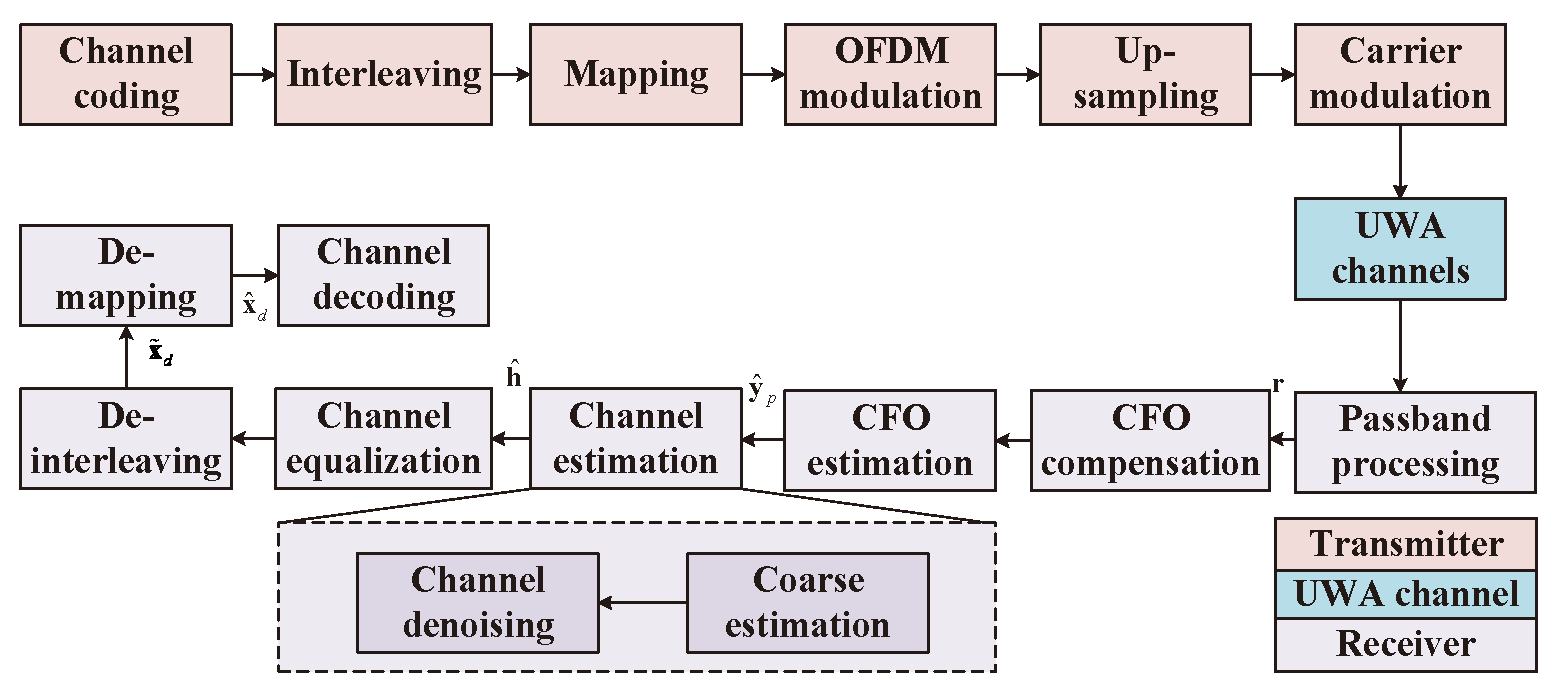
\includegraphics[width=8.5cm]{figs/flowchart.eps}
	\caption{Flowchart of OFDM.}
	\label{fig:flowchart}
\end{figure}
\par Assuming that each OFDM symbol contains $K$ subcarriers, with the $k$-th subcarrier positioned at the frequency ${f_k} = k{f_\Delta }$, where $k = 1, 2, \cdots ,K$ and ${f_\Delta }$ denotes the frequency interval. The $K$ subcarriers are categorized into $K_d$ data subcarriers and $K_p$ pilot subcarriers, with their respective index sets denoted as $\Phi_d$ and $\Phi_p$ respectively. Hence, by performing a $K$-point IDFT, each OFDM baseband signal in the time domain can be expressed as
\begin{eqnarray}\label{eq:x(n)}
	{\bf{x}}_f\left( i \right) = \frac{1}{{\sqrt K }}\left( {\sum\limits_{k \in {{\Phi}_d}} {{\bf{d}}\left( k \right){e^{j2\pi k{f_\Delta }i}}}  + \sum\limits_{k \in {{\Phi}_p}} {{\bf{d}}\left( k \right){e^{j2\pi k{f_\Delta }i}}} } \right),
\end{eqnarray}
where ${i} = 1, 2, \cdots, K$. Notation $\mathbf{d}$ denotes each mapped OFDM signal in the frequency domain, defined as ${\bf{d}} = {\left( {{d_1},{d_2}, \cdots, {d_{K}}} \right)^T}$. For the sake of convenience in derivation, subsequent derivations will utilize matrix notation ${\bf{x}}_f = {\bf{F}}_K^H{\bf{d}}$.
\par In the receiver, as detailed in~\cite{li2006ofdm}, the Doppler effect can be divided into wide-band Doppler and narrow-band Doppler. The wide-band Doppler is compensated using a resampling technique, leaving the narrow-band Doppler, which is modeled as carrier frequency offset (CFO). Accordingly, each received baseband symbol in the time domain can be expressed as ${\bf{r}} = {\bf{\Theta }}\left( {{\bf{F}}_K^H{\bf{X}}_f{{\bf{F}}_{K,\left[ {:,1:N} \right]}}{\bf{h}}} \right) + {\bf{w}}$, where ${{\bf{\Theta }}}$, ${{{\bf{X}}}}_f$, $\mathbf{h}$, and $\mathbf{w}$ denote the CFO matrix, transmitted symbol matrix, CIR matrix, and ambient noise matrix, respectively. Assuming ${{\bf{\bar \Theta }}}$ denotes the CFO compensation matrix with a tentative CFO value $\bar \varepsilon $, and the compensated signals can be expressed as
\begin{eqnarray}\label{eq:bar_r}
	{\bf{\bar r}} = {{\bf{\bar \Theta }}^H}{\bf{r}} = {{\bf{\bar \Theta }}^H}{\bf{\Theta F}}_K^H{\bf{X}}_f{{\bf{F}}_{\left[ {:,1:N} \right]}}{\bf{h}} + {{\bf{\bar \Theta }}^H}{\bf{w}}\;.
\end{eqnarray}
Subsequently, the pilot information in the frequency domain can be expressed from
\begin{eqnarray}\label{eq:yp}
	{{\bf{\bar y}}_p} &=& {{\bf{S}}_p}{{\bf{F}}_K}{\bf{\bar r}} \nonumber \\
	&=& {{\bf{S}}_p}{{\bf{F}}_K}{{\bf{\bar \Theta }}^H}{\bf{\Theta F}}_K^H{\bf{X}}_f{{\bf{F}}_{\left[ {:,1:N} \right]}}{\bf{h}} + {{\bf{S}}_p}{{\bf{F}}_K}{{\bf{\bar \Theta }}^H}{\bf{w}}\;,\\
	&=& {{\bf{A}}_p}{\bf{h}} + {{{\bf{ w}}}_p}\nonumber 
\end{eqnarray}
where $\mathbf{S}_p$ denotes the pilot selection matrix, $N$ denotes the channel length, and ${{\bf{A}}_{p}}$ denotes the observation matrix with a size of $K_p \times N$. Due to the presence of CFO interference, the matrix product ${{\bf{F}}_K}{{\bf{\bar \Theta }}^H}{\bf{\Theta F}}_K^H$ deviates from the identity matrix, with its energy becoming concentrated around the main diagonal. Consequently, it is imperative to mitigate CFO interference. In our paper, we adopt the low computational complexity one-dimensional search method as proposed in Ref.~\cite{tao2017dft}. The LS algorithm is used to estimate the channel by
\begin{eqnarray}\label{eq:LS}
	{{\bf{\bar h} }} = {\left( {{\bf{A}}_p^H{{\bf{A}}_p}} \right)^{ - 1}}{\bf{A}}_p^H{{\bf{\bar y}}_p}\;,
\end{eqnarray}
where notation $\bf{\bar h}$ denotes the estimated channel matrix, and it can be defined as ${\bf{\bar h}} = \left( {{{\bar h}_1},{{\bar h}_2}, \cdots ,{{\bar h}_N}} \right)$. Considering a linear equalizer, the output OFDM symbols can be expressed as
\begin{eqnarray}\label{eq:xbar}
	{{\bf{\bar x}}_p} = \frac{{{{\bf{\bar  y}}_p}}}{{{{\bf{F}}_{\left[ {{\Phi _p},1:L} \right]}}{\bf{\bar h}}}}\;.
\end{eqnarray}
By minimizing the squared error criterion, the CFO compensation value can be obtained by
\begin{eqnarray}\label{eq:CFO}
	\hat \varepsilon = \mathop {\arg \min }\limits_\varepsilon  \left\| {{{\bf{x}}_p} - {{{\bf{\bar x}}}_p}} \right\|_2^2\;.
\end{eqnarray}
\par After obtaining the CFO estimation $\hat \varepsilon$, the compensated pilot and data information can be expressed as $\mathbf{\hat y}_p=\mathbf{S}_p\mathbf{F}_K\mathbf{{{\bf{\hat \Theta }}}}^H\mathbf{r}$ and ${{\bf{\hat y}}_d} = {{\bf{S}}_d}{{\bf{F}}_K}{{\bf{\hat \Theta }}^H}{\bf{r}}$, where ${{\bf{\hat \Theta }}^H}$ denotes the CFO compensation matrix with a CFO compensation value $\hat \varepsilon$. Following CFO estimation and compensation, the estimated channel $\mathbf{\hat h}$ can be obtained using many channel estimation algorithms. Subsequently, channel equalization based on a linear equalizer is conducted to obtain the output data symbols by
\begin{eqnarray}\label{eq:xhar}
	{{\bf{\hat x}}_d} = \frac{{{{{\bf{\hat y}}}_d}}}{{{{\bf{F}}_{\left[ {{\Phi _d},1:L} \right]}}{\bf{\hat h}}}}\;.
\end{eqnarray}
After de-mapping and de-interleaving, the output OFDM symbols are converted into ${\bf{\tilde x}}_d$, and its length is $N_b$ times that of ${\bf{\hat x }}_d$, where $N_b$ denotes the modulation bits per symbol. The sequence ${\bf{\tilde x}}_d$ is input into the channel decoder to recover the original information.
\par Since accurate UWA channel estimation is essential to equalization and system performance, this paper focuses on improving channel estimation accuracy through physics-inspired denoising.
% =========================================================================
\section{Channel Model and Problem Formulation}
\par UWA propagation is significantly affected by dynamic underwater environments. Due to acoustic velocity gradients and water non-uniformity, reflection and refraction result in significant multipath propagation. 
\subsection{Channel Decomposition Model}\label{sec:decomposition}
\par Based on propagation mechanisms, multipath components can be categorized into direct paths, sea surface reflections, and seafloor reflections. Following~\cite{whitmarsh1963underwater}, these eigenpaths can be classified into two main types based on their temporal characteristics: static paths and dynamic paths.
\par Static paths originate from stable propagation environments, including direct paths, bottom-reflected paths, and stable refracted paths. Since water structure, seafloor topography, and sound speed profile remain relatively stable over short time scales, static paths exhibit stable time delays and slow amplitude variations, resulting in strong temporal correlation. In contrast, dynamic paths are primarily caused by sea surface reflections from time-varying, non-specular surfaces due to wind and waves. These paths exhibit dynamic time delays and fast amplitude variations, resulting in weak temporal correlation. Fig.~\ref{fig:channel_mechanisms} illustrates the propagation mechanisms of static and dynamic paths.


\begin{figure}[htbp]
	\centering
	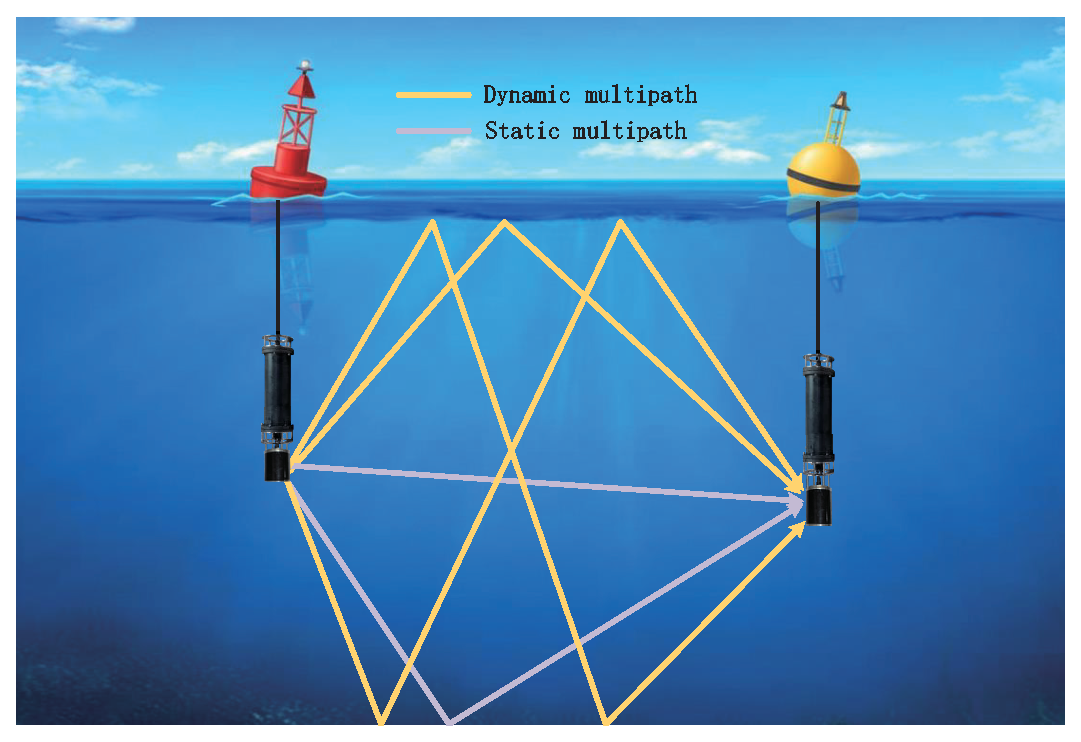
\includegraphics[width=8cm]{figs/channel_mechanisms.eps}
	\caption{Schematic diagram of channel mechanisms.}
	\label{fig:channel_mechanisms}
\end{figure}

\par Consequently, we can establish UWA channel mathematical model based on static and dynamic paths decouple. Let $N$ denotes channel length and the $t$ time slot channel impulse respond in the time domain $\mathbf{h}^T\in\mathbb{C}^{N\times 1}$ can be expressed as 
\begin{equation}\label{eq:h}
	{{\bf{h}}^T}\left( t \right) = {\bf{h}}_s^T\left( t \right) + {\bf{h}}_d^T\left( t \right)\;,
\end{equation}
where $\mathbf{h}_s\in\mathbb{C}^{N\times 1}$ and $\mathbf{h}_d\in\mathbb{C}^{N\times 1}$ denote static and dynamic channels respectively. Subsequently, considering the channel matrix ${\mathbf{H}} \in {^{N \times M}}$ with a observation window of $M$ can be expressed as
\begin{equation}\label{eq:H}
	\begin{array}{l}
		{{\bf{H}}^T} = {\bf{H}}_s^T + {\bf{H}}_d^T\;\\
		\left[ {\begin{array}{*{20}{c}}
				{{{\bf{h}}^T}\left( t \right)}\\
				{{{\bf{h}}^T}\left( {t + 1} \right)}\\
				\cdots \\
				{{{\bf{h}}^T}\left( {t + M} \right)}
		\end{array}} \right] = \left[ {\begin{array}{*{20}{c}}
				{{\bf{h}}_s^T\left( t \right)}\\
				{{\bf{h}}_s^T\left( {t + 1} \right)}\\
				\cdots \\
				{{\bf{h}}_s^T\left( {t + M} \right)}
		\end{array}} \right] + \left[ {\begin{array}{*{20}{c}}
				{{\bf{h}}_d^T\left( t \right)}\\
				{{\bf{h}}_d^T\left( {t + 1} \right)}\\
				\cdots \\
				{{\bf{h}}_d^T\left( {t + M} \right)}
		\end{array}} \right]
	\end{array}\;.
\end{equation}
\subsection{Static and dynamic channel characteristics}\label{sec:channel_characteristic}
\par In this subsection, we provide the static and dynamic channel characteristics in terms of time domain and delay domain, respectively based on physics mechanisms.
\subsubsection{Delay Domain}
\par From the delay domain, i.e., considering one time slot UWA channel as shown in Eq.~\eqref{eq:h}. The UWA channel exhibits significant sparsity characteristic, it can be expressed as $\kappa  \ll N$, where $\kappa$ and $N$ denotes the non-zero elements in UWA channel and channel length respectively. The static and dynamic channel is one part of UWA channels, obviously, the both sub-channels also exhibits significant sparsity, i.e.,
\begin{eqnarray}
	\begin{array}{l}
		{\kappa _s} \ll N\\
		{\kappa _d} \ll N
	\end{array}
\end{eqnarray}
where $\kappa _s$ and $\kappa _d$ denote the non-zero elements of static channel and dynamic channel respectively, and they satisfy $\kappa =\kappa _s+\kappa _d$.
\subsubsection{Time Domain}
\begin{figure}[htbp]
	\centering
	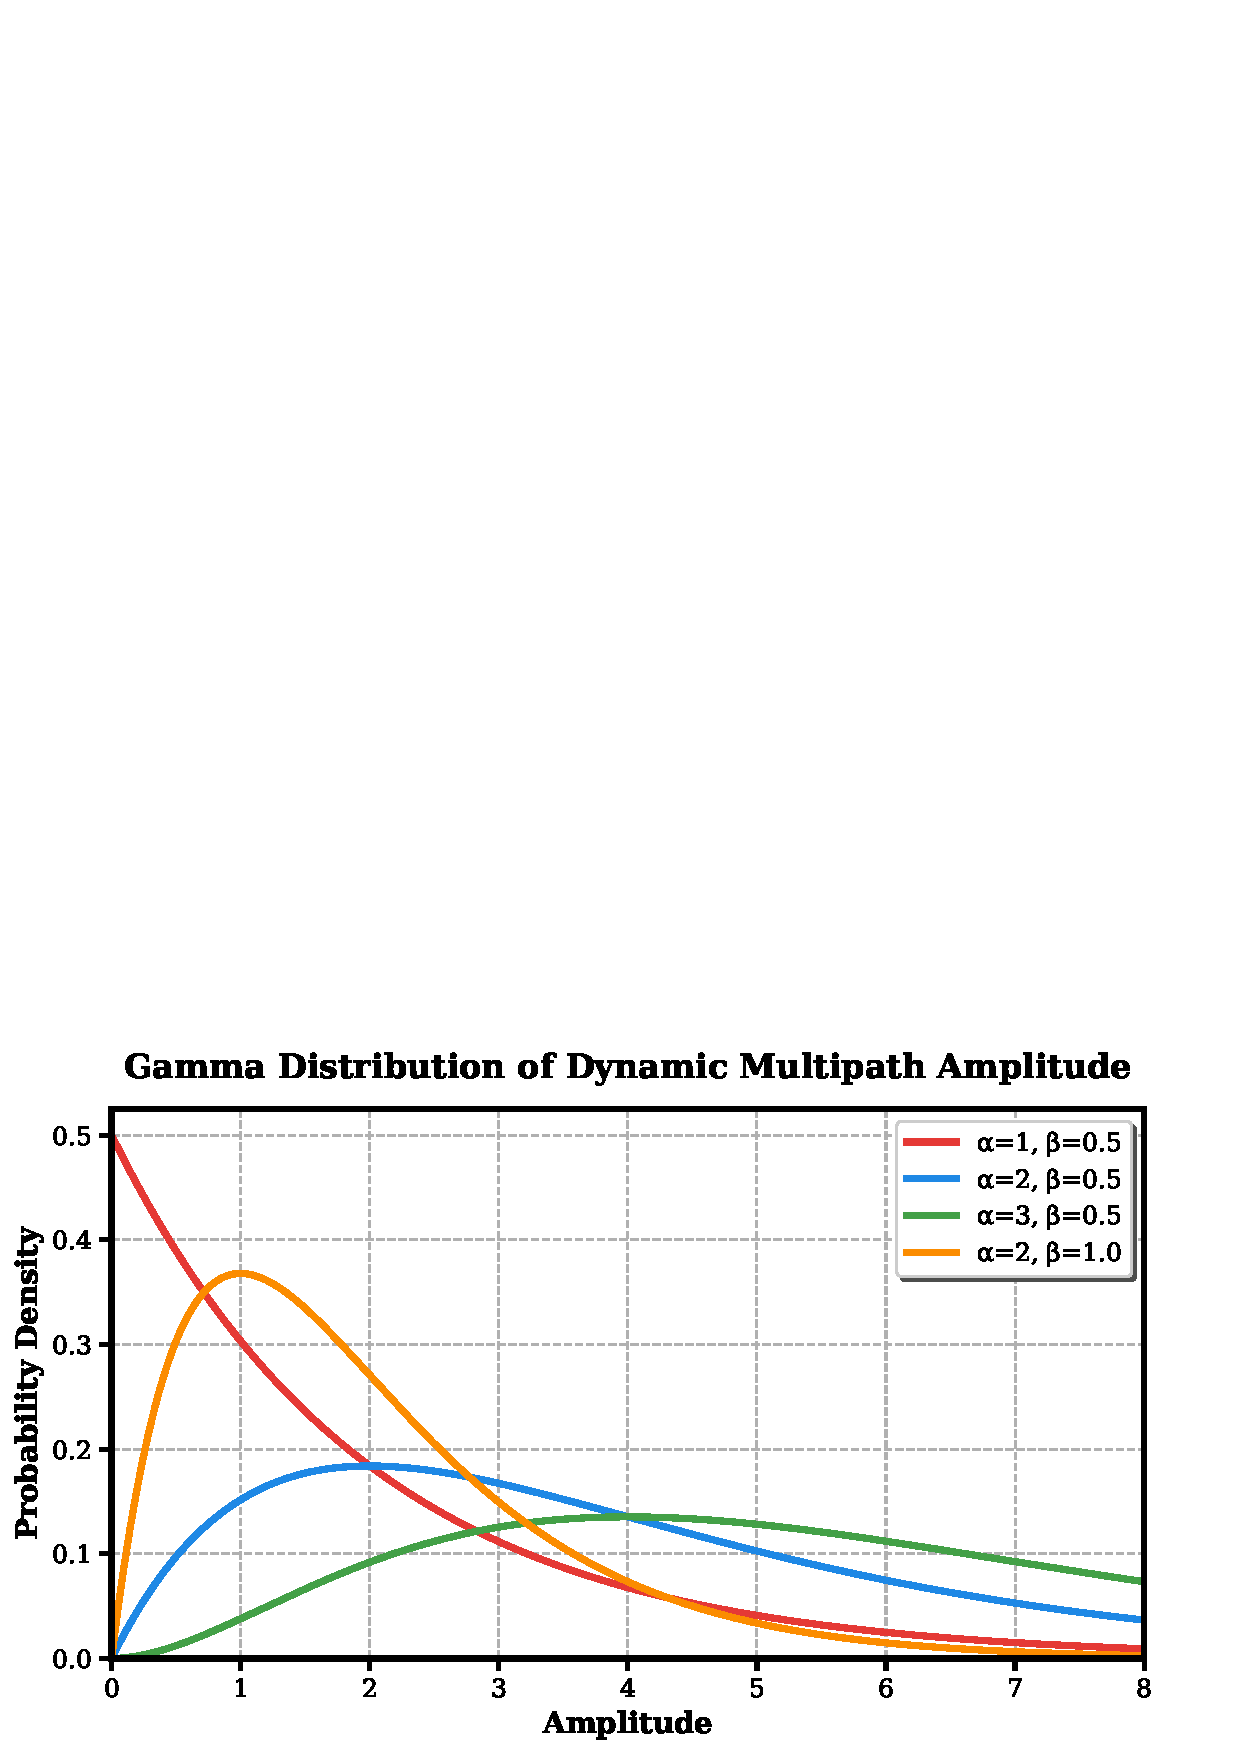
\includegraphics[width=8cm]{figs/Gamma.pdf}
	\caption{Gamma distribution of dynamic multipath amplitude.}
	\label{fig:Gamma}
\end{figure}
\par UWA channels exhibit significant time-varying characteristics. Experimental results~\cite{jiang2022exploiting, zhou2017exploiting, jiang2021exploiting} indicate that the envelope distribution of the received signal in the direct path follows Gaussian distribution, while the surface reflected path exhibits Gamma distribution, as shown in Fig.~\ref{fig:Gamma}, particularly at large grazing angles. Consequently, considering each multipath component of the static component in the time domain, the amplitude time-varying characteristic can be expressed as:
\begin{equation}
{a_s}\left( \tau  \right) \sim {\cal N} \left( {{\mu _s},\sigma _s^2} \right)\;,
\end{equation}
where $a_s$ denotes the amplitude of CIR, and $\mathcal{N}(\mu_s, \sigma_s^2)$ denotes Gaussian distribution with mean $\mu_s$ and variation $\sigma_s$. Due to the water body and seafloor remain stable, the delay of multipath is remain stable, and it can be expressed as 
\begin{equation}
	\Upsilon {}_s\left( {t + 1} \right) = \Upsilon {}_s\left( t \right)
\end{equation}
where $\Upsilon (t)$ denotes the index set of static in the $t$ slot.
\par Focusing on dynamic multipath caused by dynamic sea surface, considering each multipath component of the dynamic component in the time domain, the amplitude time-varying characteristic can be expressed as:
\begin{equation}
{a_d}\left( \tau  \right) \sim \Gamma ({\alpha _d},{\beta _d}),
\end{equation}
where $\Gamma ({\alpha _d},{\beta _d})$ denotes Gamma distribution with shape parameter $\alpha_d$ and inverse scale parameter $\beta_d$. Due to the rapid motion of sea surface waves, the positions of reflection points undergo significant and rapid changes, resulting in substantial jitter in the propagation time delay of the paths. Hence, the time delay variation is modeled as a random perturbation, implemented by adding a zero-mean random variable $\mu_d=0$ to the Bellhop-generated fixed path delay. The variance of this variable $\sigma_d$ dictates the intensity of the resultant fluctuation. 
\par From the aspect of temporal correlation, for static component, due to stable water structure, seafloor topography, sediment composition, and SSP in short time. Hence, the channel of the adjacent moment has a strong correlation and can be expressed as 
\begin{eqnarray}
	\mathbb{E}[\|\mathbf{H}_{\mathrm{s}}(t+\Delta t)-\mathbf{H}_{\mathrm{s}}(t)\|_F^2] \approx 0\;,
\end{eqnarray}
where $\Delta t \le {T_c}$, and $T_c$ denotes channel correlation time. As for dynamic component, because sea surface exhibits significantly dynamic characteristic, hence, the channel of the adjacent moment has a strong correlation and can be expressed as  
\begin{eqnarray}
\mathbb{E}[{{\bf{H}}_{d}}(t + \Delta t){\bf{H}}_d^T(t)] \approx 0\;.
\end{eqnarray}

%\par In summary, the key properties can be summarized as follows:
%\begin{itemize}
%	\item \textbf{Sparsity}: When $L_s \ll \min(M,N)$, $\bm{H}_{\mathrm{s}}$ has sparse representation in angular domain via DFT matrix $\bm{F}$: $\|\bm{F}^H\bm{H}_{\mathrm{s}}\bm{F}\|_0 \ll MN$.
%	\item \textbf{Low-Rank}: $L_d \ll \min(M,N)$, $\text{rank}(\bm{H}_{\mathrm{d}}) \leq L_d$.
%	\item \textbf{Temporal Correlation}: For static component, $\mathbb{E}[\|\bm{H}_{\mathrm{s}}(t+\Delta t)-\bm{H}_{\mathrm{s}}(t)\|_F^2] \approx 0$ when $\Delta t \ll T_{\text{static}}$.
%\end{itemize}



%\begin{equation}
%	{{\bf{h}}_{\rm{s}}}(t) = \sum\limits_{i = 0}^{{N_s} - 1} {{{\bf{a}}_s}\left( i \right)\delta \left( {t - {\tau _i}} \right)} 
%\end{equation}
%where ${\delta \left( {t} \right)}$ denotes the impulse function, ${{\tau _i}}$ denotes the $i$-th multipath delay in the $t$ timeslot, $N_s$ denotes the number of multipath. Notation $\mathbf{a}_s$ denotes the amplitude of CIR, and it satisfies Gaussian distribution, which can be expressed as

%\subsection{Noisy Observation Model}
%\par The receiver obtains LS channel estimate through orthogonal pilot transmission:
%\begin{equation}
%\widetilde{\bm{H}}=\bm{H}+\bm{N}=\bm{H}_{\mathrm{s}}+\bm{H}_{\mathrm{d}}+\bm{N},
%\end{equation}
%where $\bm{N}\sim\mathcal{CN}(\bm{0},\sigma_n^2\bm{I}_{MN})$ is additive white Gaussian noise. The signal-to-noise ratio is defined as
%\begin{equation}
%\text{SNR}=10\log_{10}\frac{\mathbb{E}[\|\bm{H}\|_F^2]}{\mathbb{E}[\|\bm{N}\|_F^2]}=10\log_{10}\frac{\|\bm{H}\|_F^2}{MN\sigma_n^2}.
%\end{equation}

%% 问题建立
\subsection{Optimization Problem}
\par Since estimated channels inevitably suffer from noise interference, accurate channel estimation is essential for OFDM system performance. Our goal is to improve channel estimation accuracy through denoising. The optimization problem can be formulated as 
\begin{equation}
\mathop {\min }\limits_{{\bf{\hat H}}} \mathbb{E} \left[ {\left\| {{\bf{H}} - {\bf{\hat H}}} \right\|_F^2} \right]\;.
\end{equation}
\par Conventional deep learning methods treat the channel matrix as a single entity without exploiting physical characteristics. Based on the analysis in Section~\ref{sec:decomposition} and~\ref{sec:channel_characteristic}, UWA channels can be decomposed into static and dynamic components. We reformulate the optimization problem to jointly estimate these components:
\begin{equation}
\begin{aligned}
&\mathop {\min }\limits_{{{{\bf{\hat H}}}_{\rm{s}}},{{{\bf{\hat H}}}_d}} \mathbb{E} \left[ {\underbrace {\left\| {{{\bf{H}}_s} - {{{\bf{\hat H}}}_s}} \right\|_F^2}_{{\rm{static MSE}}} + \underbrace {\left\| {{{\bf{H}}_d} - {{{\bf{\hat H}}}_d}} \right\|_F^2}_{{\rm{dynamic MSE}}}} \right]\\
&\text{subject to:}\quad\hat{\mathbf{H}}_{\mathrm{s}}\in\mathcal{S},\quad\hat{\mathbf{H}}_{\mathrm{d}}\in\mathcal{D},
\end{aligned}
\label{eq:optimization}
\end{equation}
where $\mathcal{S}$ denotes the space of sparse matrices and $\mathcal{D}$ denotes low-rank matrices. The final estimate is $\hat{\mathbf{H}}=\hat{\mathbf{H}}_{\mathrm{s}}+\hat{\mathbf{H}}_{\mathrm{d}}$.

\par Problem~\eqref{eq:optimization} is ill-posed without prior knowledge. Classical approaches assume known sparsity level or rank, which are unavailable in practice. Moreover, the static-dynamic ambiguity makes decomposition non-unique without additional constraints.

% =========================================================================
\section{Theoretical Foundations}
\par Before describing DSS-Net, we establish theoretical connections to sparse recovery and low-rank matrix completion that motivate our physics-informed loss function design. 

\subsection{Sparse Recovery Framework}
\par Consider the angular-domain representation of static component via $M\times M$ DFT matrix $\mathbf{F}_M$ and $N\times N$ DFT matrix $\mathbf{F}_N$:
\begin{equation}
\mathbf{X}_{\mathrm{s}}=\mathbf{F}_M^H\mathbf{H}_{\mathrm{s}}\mathbf{F}_N,
\end{equation}
where $\mathbf{X}_{\mathrm{s}}$ is approximately $k$-sparse with $k \ll MN$. The observation model becomes
\begin{equation}
\widetilde{\mathbf{H}}=\mathbf{F}_M\mathbf{X}_{\mathrm{s}}\mathbf{F}_N^H+\mathbf{H}_{\mathrm{d}}+\mathbf{N}\;,
\end{equation}
where $\mathbf{N}$ denotes background noise. If the sensing operator $\mathcal{A}(\mathbf{X})=\mathbf{F}_M\mathbf{X}\mathbf{F}_N^H$ satisfies restricted isometry property (RIP) of order $2k$ with constant $\delta_{2k}<\sqrt{2}-1$ \cite{Candes2005Decoding}, then $\ell_1$ minimization
\begin{equation}
\min_{\mathbf{X}}\|\mathbf{X}\|_1\quad\text{s.t.}\quad\|\widetilde{\mathbf{H}}-\mathbf{F}_M\mathbf{X}\mathbf{F}_N^H-\mathbf{H}_{\mathrm{d}}\|_F\leq\epsilon
\end{equation}
recovers $\mathbf{X}_{\mathrm{s}}$ with error $\|\mathbf{X}_{\mathrm{s}}-\hat{\mathbf{X}}_{\mathrm{s}}\|_F\leq C\sigma_n\sqrt{k\log(MN)}$ for constant $C$ depending on $\delta_{2k}$ \cite{Candes2006Stable}.

\par The $\ell_1$ term in our loss function serves as a convex relaxation of the sparsity constraint, enabling stable recovery under noise.

\subsection{Low-Rank Matrix Recovery}

For dynamic component with rank $r \ll \min(M,N)$, consider the nuclear norm minimization:
\begin{equation}
\min_{\mathbf{X}}\|\mathbf{X}\|_*\quad\text{s.t.}\quad\|\widetilde{\mathbf{H}}-\mathbf{H}_{{s}}-\mathbf{X}\|_F\leq\epsilon,
\end{equation}
where $\|\mathbf{X}\|_*=\sum_i\sigma_i(\mathbf{X})$ is the sum of singular values. Under incoherence conditions \cite{Candes2009Exact}, this recovers $\mathbf{H}_{{d}}$ exactly when number of observations exceeds $O(r(M+N)\log^2(MN))$.

The nuclear norm gradient has simple form \cite{Watson1992Characterization}:
\begin{equation}
\nabla_{\mathbf{X}}\|\mathbf{X}\|_*=\mathbf{U}\mathbf{V}^H,
\end{equation}
where $\mathbf{X}=\mathbf{U}\mathbf{\Sigma}\mathbf{V}^H$ is the SVD, enabling efficient back propagation in our network.

\subsection{Separation via Orthogonality}

To ensure unique decomposition, we enforce low correlation between static and dynamic components. Define correlation:
\begin{equation}
\rho(\mathbf{H}_{\mathrm{s}},\mathbf{H}_{\mathrm{d}})=\frac{|\langle\mathbf{H}_{\mathrm{s}},\mathbf{H}_{\mathrm{d}}\rangle_F|}{\|\mathbf{H}_{\mathrm{s}}\|_F\|\mathbf{H}_{\mathrm{d}}\|_F},
\end{equation}
where $\langle\mathbf{A},\mathbf{B}\rangle_F=\text{tr}(\mathbf{A}^H\mathbf{B})$ is Frobenius inner product. Minimizing $\rho$ encourages near-orthogonal decomposition, reducing ambiguity.

\textit{Proposition 1:} If $\mathbf{H}_{\mathrm{s}}$ is $k$-sparse in angular domain and $\mathbf{H}_{\mathrm{d}}$ has rank $r$ with incoherent singular vectors, then $\rho(\mathbf{H}_{\mathrm{s}},\mathbf{H}_{\mathrm{d}})\leq\sqrt{kr/MN}$ with high probability under random scatterer distribution.

\par This result justifies our separation quality loss, which minimizes correlation between estimated components. The proof is provided in Appendix~A.

% =========================================================================
\section{DSS-Net Architecture}
%\par The DSS-Net is included into the receiver of UWA communication systems, as shown in the upper part of Fig.~\ref{fig:DSS-Net}. The DSS-Net is focusing on optimize the output estimated channel, which improving the equalization performance.

\begin{figure*}[htbp]
	\centering
	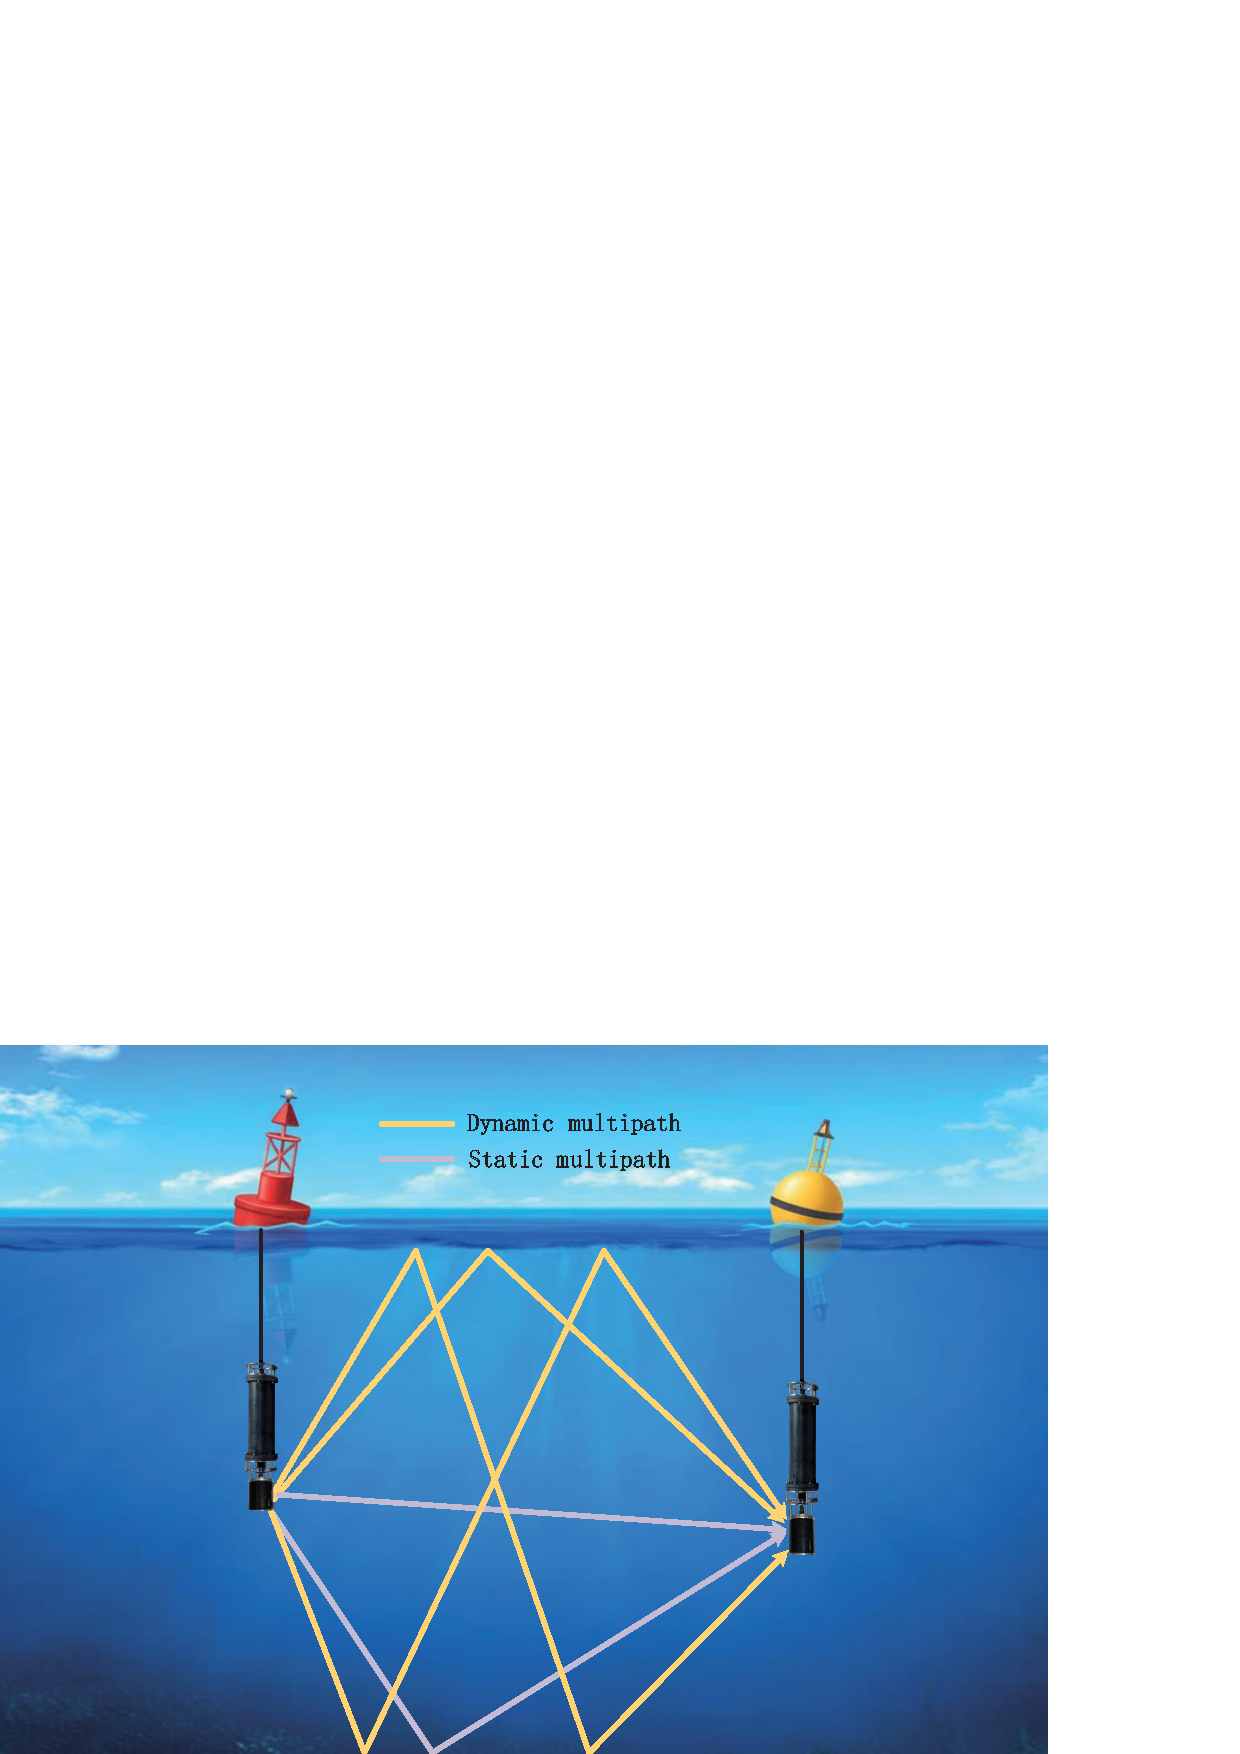
\includegraphics[width=15cm]{figs/channel_mechanisms.jpg}
	\caption{Schematic diagram of DSS-Net.}
	\label{fig:DSS-Net}
\end{figure*}

\subsection{Network Overview}
\par DSS-Net adopts a U-Net encoder-decoder architecture~\cite{Ronneberger2015UNet} with three key innovations: (i) shared encoder extracting common features; (ii) dual symmetric decoders for parallel reconstruction; (iii) squeeze-and-excitation (SE) attention at the bottleneck~\cite{Hu2018SqueezeExcitation}. The architecture is illustrated in Fig.~\ref{fig:DSS-Net}.

\par \textit{Input Representation:} The complex channel $\widetilde{\mathbf{H}}\in\mathbb{C}^{M\times N}$ is decomposed into real and imaginary parts:
\begin{equation}
\mathbf{X}_{\text{in}}=[\Re(\widetilde{\mathbf{H}});\Im(\widetilde{\mathbf{H}})]\in\mathbb{R}^{2\times M\times N}.
\end{equation}

\par \textit{Encoder:} Four downsampling blocks with channel dimensions $64\to128\to256\to512\to512$. Each block contains:
\begin{equation}
\begin{aligned}
\bm{z}_1&=\text{BN}(\text{LeakyReLU}(\text{Conv}_{3\times 3}(\bm{x}))),\\
\bm{z}_2&=\text{BN}(\text{LeakyReLU}(\text{Conv}_{3\times 3}(\bm{z}_1))),\\
\bm{x}_{\text{down}}&=\text{MaxPool}_{2\times 2}(\bm{z}_2).
\end{aligned}
\end{equation}
Skip connections preserve $\{\bm{z}_2^{(i)}\}_{i=1}^4$ for decoder reconstruction.

\par \textit{Attention Bottleneck:} At the deepest layer, the SE module computes channel-wise attention:
\begin{equation}
\begin{aligned}
\bm{s}&=\text{GAP}(\bm{z}_{\text{bottleneck}})\in\mathbb{R}^{512},\\
\bm{w}&=\sigma(\bm{W}_2\delta(\bm{W}_1\bm{s}+\bm{b}_1)+\bm{b}_2),\\
\bm{z}_{\text{attn}}&=\bm{z}_{\text{bottleneck}}\odot\bm{w},
\end{aligned}
\end{equation}
where GAP is global average pooling, $\delta$ is ReLU, $\sigma$ is sigmoid, $\bm{W}_1\in\mathbb{R}^{64\times512}$, $\bm{W}_2\in\mathbb{R}^{512\times64}$ (reduction ratio 8).

\par \textit{Decoders:} Two structurally identical decoders with upsampling:
\begin{equation}
\begin{aligned}
\bm{z}_{\text{up}}&=\text{ConvTranspose}_{2\times 2}(\bm{z}),\\
\bm{z}_{\text{cat}}&=[\bm{z}_{\text{up}};\bm{z}_{\text{skip}}],\\
\bm{z}_{\text{out}}&=\text{DoubleConv}(\bm{z}_{\text{cat}}).
\end{aligned}
\end{equation}
Final outputs are two-channel maps converted to complex:
\begin{equation}
\hat{\bm{H}}_{\mathrm{s}}=\bm{Y}_{\mathrm{s}}^{(1)}+j\bm{Y}_{\mathrm{s}}^{(2)},\quad\hat{\bm{H}}_{\mathrm{d}}=\bm{Y}_{\mathrm{d}}^{(1)}+j\bm{Y}_{\mathrm{d}}^{(2)}.
\end{equation}

\subsection{Design Rationale}

\par \textit{Parameter Sharing:} The shared encoder reduces parameters compared to two independent encoders while learning common low-level features.

\par \textit{Symmetric Decoders:} Our symmetric design (43.6M parameters vs. 62M for dual full networks) avoids bias toward either component and achieves 42\% parameter reduction.

\par \textit{Attention Mechanism:} The SE module enables adaptive feature selection, emphasizing informative frequency bands for static-dynamic separation.

\subsection{Computational Complexity}

\par Per-sample complexity is dominated by convolutions:
\begin{equation}
\mathcal{C}=\sum_{l=1}^{L}K_l^2C_{\text{in}}^{(l)}C_{\text{out}}^{(l)}H_lW_l,
\end{equation}
where $K_l$ is kernel size, $C$ are channels, $H_l,W_l$ are spatial dimensions at layer $l$. For our architecture with $M=100,N=150$:
\begin{equation}
\mathcal{C}\approx9\times64^2\times100\times150\approx5.5\text{ GFLOPs}.
\end{equation}
This enables real-time processing at $>$180 FPS on NVIDIA A100 GPU.

% =========================================================================
\section{Physics-Informed Loss Function}

\par We design a multi-term objective function embedding domain knowledge from UWA channel physics.

\subsection{Weighted Reconstruction Loss}

\par The primary objective ensures fidelity to ground truth:
\begin{multline}
\mathcal{L}_{\text{recon}}=\frac{1}{B}\sum_{b=1}^{B}\Bigl[\alpha_{\mathrm{s}}\|\hat{\mathbf{H}}_{\mathrm{s}}^{(b)}-\mathbf{H}_{\mathrm{s}}^{(b)}\|_F^2\\
+\alpha_{\mathrm{d}}\|\hat{\mathbf{H}}_{\mathrm{d}}^{(b)}-\mathbf{H}_{\mathrm{d}}^{(b)}\|_F^2+\alpha_{\mathrm{t}}\|\hat{\mathbf{H}}^{(b)}-\mathbf{H}^{(b)}\|_F^2\Bigr],
\end{multline}
where $\hat{\mathbf{H}}=\hat{\mathbf{H}}_{\mathrm{s}}+\hat{\mathbf{H}}_{\mathrm{d}}$. We set $\alpha_{\mathrm{s}}=1$, $\alpha_{\mathrm{d}}=2$, $\alpha_{\mathrm{t}}=3$ to prioritize total channel accuracy while ensuring component-level supervision.

The hierarchy $\alpha_{\mathrm{t}}>\alpha_{\mathrm{d}}>\alpha_{\mathrm{s}}$ reflects that: (i) end-to-end performance depends on total channel; (ii) dynamic component is harder to estimate due to rapid variation; (iii) static component is easier given its smoothness.

\subsection{Sparsity-Promoting Regularization}

\par To encourage sparse static component:
\begin{equation}
\mathcal{L}_{\text{sparse}}=\frac{1}{B}\sum_{b=1}^{B}\|\hat{\mathbf{H}}_{\mathrm{s}}^{(b)}\|_1=\frac{1}{B}\sum_{b=1}^{B}\sum_{m,n}|\hat{H}_{\mathrm{s},mn}^{(b)}|.
\end{equation}

From sparse recovery theory \cite{Candes2005Decoding}, $\ell_1$ minimization provably recovers sparse signals under RIP. Our weak regularization ($\lambda_{\text{sparse}}=10^{-4}$) provides soft constraint without over-constraining.

\subsection{Nuclear Norm Regularization}

\par To promote low-rank dynamic component:
\begin{equation}
\mathcal{L}_{\text{rank}}=\frac{1}{B}\sum_{b=1}^{B}\|\hat{\mathbf{H}}_{\mathrm{d}}^{(b)}\|_*=\frac{1}{B}\sum_{b=1}^{B}\sum_{i=1}^{\min(M,N)}\sigma_i(\hat{\mathbf{H}}_{\mathrm{d}}^{(b)}),
\end{equation}
where $\sigma_i$ are singular values. Nuclear norm is tightest convex relaxation of matrix rank \cite{Recht2010Guaranteed}.

Implementation: We compute SVD in float32 for numerical stability:
\begin{equation}
\hat{\mathbf{H}}_{\mathrm{d}}^{\text{fp32}}=\mathbf{U}\mathbf{\Sigma}\mathbf{V}^H,\quad\nabla_{\hat{\mathbf{H}}_{\mathrm{d}}}\|\hat{\mathbf{H}}_{\mathrm{d}}\|_*=\mathbf{U}\mathbf{V}^H.
\end{equation}

\subsection{Temporal Correlation Loss}

\par We exploit different temporal characteristics of static and dynamic components.

\par \textit{Static Smoothness:} Penalize large temporal variations:
\begin{equation}
\mathcal{L}_{\text{temp}}^s=\frac{1}{B}\sum_{b=1}^{B}\sum_{i}\|[\hat{\mathbf{H}}_{\mathrm{s}}^{(b)}]_{:,i+1}-[\hat{\mathbf{H}}_{\mathrm{s}}^{(b)}]_{:,i}\|_2^2,
\end{equation}
where subscript $:,i$ denotes $i$-th column (frequency or spatial dimension).

\par \textit{Dynamic Variation:} Encourage moderate change via hinge loss:
\begin{equation}
\mathcal{L}_{\text{temp}}^d=\frac{1}{B}\sum_{b=1}^{B}\max\Bigl(0,\epsilon-\sum_{i}\|[\hat{\mathbf{H}}_{\mathrm{d}}^{(b)}]_{:,i+1}-[\hat{\mathbf{H}}_{\mathrm{d}}^{(b)}]_{:,i}\|_2^2\Bigr),
\end{equation}
with threshold $\epsilon=0.01$. This prevents trivial solutions where $\hat{\mathbf{H}}_{\mathrm{d}}\approx 0$.

Total temporal loss: $\mathcal{L}_{\text{temp}}=\mathcal{L}_{\text{temp}}^s+\mathcal{L}_{\text{temp}}^d$.

\subsection{Separation Quality Metric}

\par To avoid degenerate solutions where both decoders output similar matrices, we minimize correlation:
\begin{equation}
\mathcal{L}_{\text{sep}}=-\frac{1}{B}\sum_{b=1}^{B}\rho(\hat{\mathbf{H}}_{\mathrm{s}}^{(b)},\hat{\mathbf{H}}_{\mathrm{d}}^{(b)}),
\end{equation}
where Pearson correlation is
\begin{equation}
\rho(\mathbf{A},\mathbf{B})=\frac{\langle\mathbf{A}-\bar{\mathbf{A}},\mathbf{B}-\bar{\mathbf{B}}\rangle_F}{\|\mathbf{A}-\bar{\mathbf{A}}\|_F\|\mathbf{B}-\bar{\mathbf{B}}\|_F},
\end{equation}
with $\bar{\mathbf{A}}=\frac{1}{MN}\sum_{mn}A_{mn}$ being mean. Negative sign ensures lower correlation yields smaller loss.

\subsection{Total Objective}

\par Combining all terms:
\begin{equation}
\begin{aligned}
\mathcal{L}_{\text{total}}=&\mathcal{L}_{\text{recon}}+\lambda_{\text{sparse}}\mathcal{L}_{\text{sparse}}+\lambda_{\text{rank}}\mathcal{L}_{\text{rank}}\\
&+\lambda_{\text{temp}}\mathcal{L}_{\text{temp}}+\lambda_{\text{sep}}\mathcal{L}_{\text{sep}},
\end{aligned}
\end{equation}
with hyperparameters $\lambda_{\text{sparse}}=\lambda_{\text{rank}}=10^{-4}$, $\lambda_{\text{temp}}=10^{-2}$, $\lambda_{\text{sep}}=5\times10^{-2}$ tuned via validation.

\par In contrast, standard single-decoder U-Net uses only $\mathcal{L}_{\text{MSE}}=\|\hat{\mathbf{H}}-\mathbf{H}\|_F^2$, without physics-informed guidance from decomposition structure, sparsity/low-rank priors, and temporal correlation.

% =========================================================================
%\section{Dataset and Implementation}
\section{Simulation Experiments}
\par We evaluate DSS-Net against baseline methods including no processing, SVD truncation~\cite{suresh2017two}, Wavelet Shrinkage~\cite{Donoho1995Wavelet}, CResNet~\cite{CResNet_TWC21}, DnCNN~\cite{Zhang2017DnCNN}, and U-Net~\cite{wei2021physics}. Performance is evaluated using normalized mean squared error (NMSE) and bit error rate (BER). The NMSE is defined as:
\begin{equation}
	\text{NMSE}_{\text{dB}}=10\log_{10}\frac{\|\mathbf{H}-\hat{\mathbf{H}}\|_F^2}{\|\mathbf{H}\|_F^2}\;.
\end{equation}
\subsection{Ray-Tracing Channel Generation}
\par We use the Bellhop ray-tracing model~\cite{bellhop} to generate UWA channel impulse responses (CIRs). The channel matrix is constructed following the decomposition model in Section~\ref{sec:decomposition}. Table~\ref{tab:Bellhop} lists the simulation parameters. Transmitter and receiver depths range from 0.5~m to 13.5~m in 15~m water depth, with horizontal distances from 0.5~km to 5~km. The sound speed profile (SSP), shown in Fig.~\ref{fig:S_SSP}, is derived from sea trial measurements in Xiamen Harbor. Fig.~\ref{fig:S_channel} shows an example CIR with complex multipath structure and maximum delay of 28.75~ms.
\begin{table}[!htbp]
	\caption{\textsc{Ray-Tracing Dataset Generation Parameters.} Channel impulse responses are generated using the Bellhop acoustic ray-tracing model with the sound speed profile measured in Xiamen Harbor. Static and dynamic multipath components are distinguished by reflection counts from sea floor and sea surface, respectively.}
	\label{tab:Bellhop}
	\centering
	\setlength{\tabcolsep}{4pt}
	\renewcommand\arraystretch{1.15}
	\small
	\begin{tabular}{p{165pt} >{\centering\arraybackslash}p{25pt} >{\centering\arraybackslash}p{50pt}}
		\toprule[1.5pt]
		\rowcolor{tableheader}
		\textbf{Parameter} & \textbf{Symbol} & \textbf{Value}\\
		\midrule[1pt]
		\rowcolor{tablerow1}
		Depth of transmitter (m)	&$L_{T}$	& 0.5 -- 13.5 \\
		\rowcolor{tablerow2}
		Depth of receiver (m)		&$L_{R}$	& 0.5 -- 13.5 \\
		\rowcolor{tablerow1}
		Depth of water (m)			&$L_W$	& 15 \\
		\rowcolor{tablerow2}
		Horizontal distances (km)	&$L_0$	& 0.5 -- 5 \\
		\midrule[0.5pt]
		\rowcolor{tablerow1}
		Mean of static amplitude	&$\mu_s$	& 0	\\
		\rowcolor{tablerow2}
		Variance of static amplitude	&$\sigma_s^2$			& 0.1 \\
		\midrule[0.5pt]
		\rowcolor{tablerow1}
		Gamma shape (dynamic)  &$\alpha_d$	& 0.5	\\
		\rowcolor{tablerow2}
		Gamma inverse scale (dynamic) &$\beta_d$	& 0.3	\\
		\rowcolor{tablerow1}
		Mean of dynamic delay &$\mu_d$					& 0	\\
		\rowcolor{tablerow2}
		Variance of dynamic delay				&$\sigma_d^2$			& 0.4 \\
		\bottomrule[1.5pt]
	\end{tabular}
	\renewcommand\arraystretch{1.0}
\end{table}
\begin{figure}[!htbp]
	\centering
	\subfloat[\label{fig:S_SSP}]
	{
		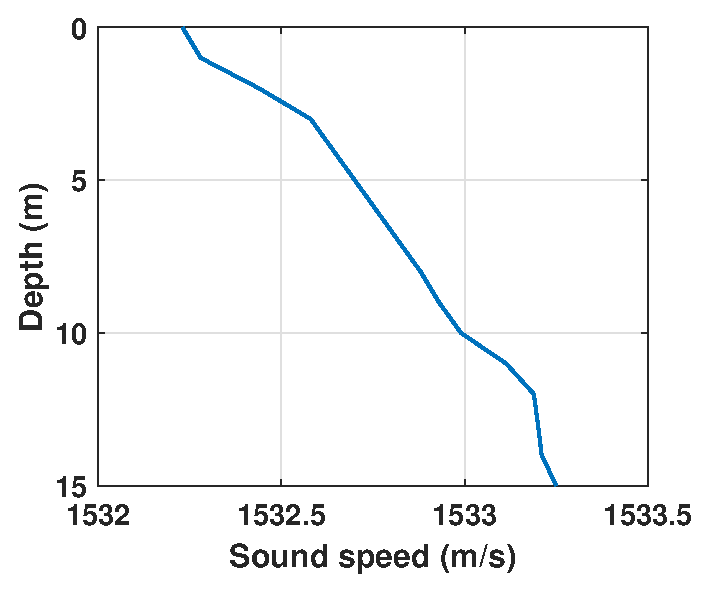
\includegraphics[width=4.2cm]{figs/Bellhop_SSP.eps}
	}
	\subfloat[\label{fig:S_channel}]
	{
		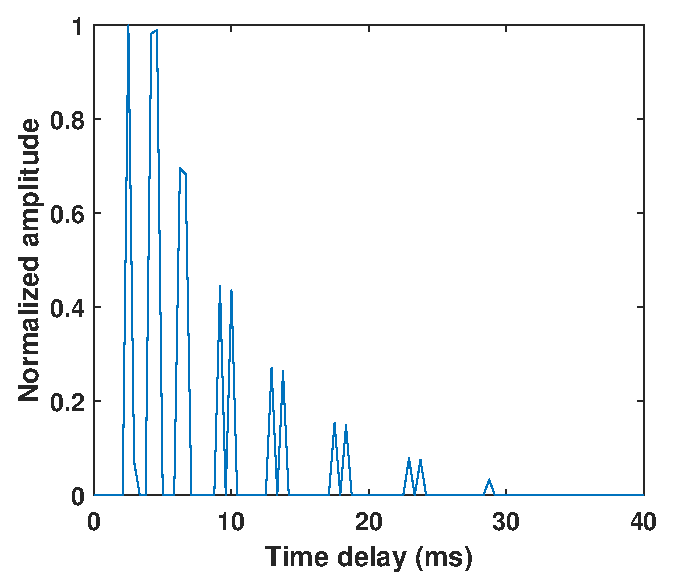
\includegraphics[width=4cm]{figs/Bellhop.eps}
	}
	\caption{Simulation environments. (a) SSP obtained in Xiamen Harbor. (b) Simulated UWA channel.}
	\label{fig:Bellhop}
\end{figure}

\par To generate the channel matrix based on the CIR generating by the Bellhop model, we adopt the channel model and characteristics analysis in Section~\ref{sec:decomposition}. The relative parameters are also shown in Table~\ref{tab:Bellhop}. The static and dynamic multipath determination depends on the output reflection counts caused by sea floor and sea surface in the Bellhop model. A sample of channel matrix based on the CIR shown in Fig.~\ref{fig:S_channel} and its decomposition is shown in Fig.~\ref{fig:matrix}, showing the characteristic of static and dynamic in the time domain. This yields supervised triplets $(\mathbf{H}_s,\mathbf{H}_d,\mathbf{H})$ for training.

\begin{figure}[!htbp]
	\centering
	\subfloat[\label{fig:All_channel}]
	{
		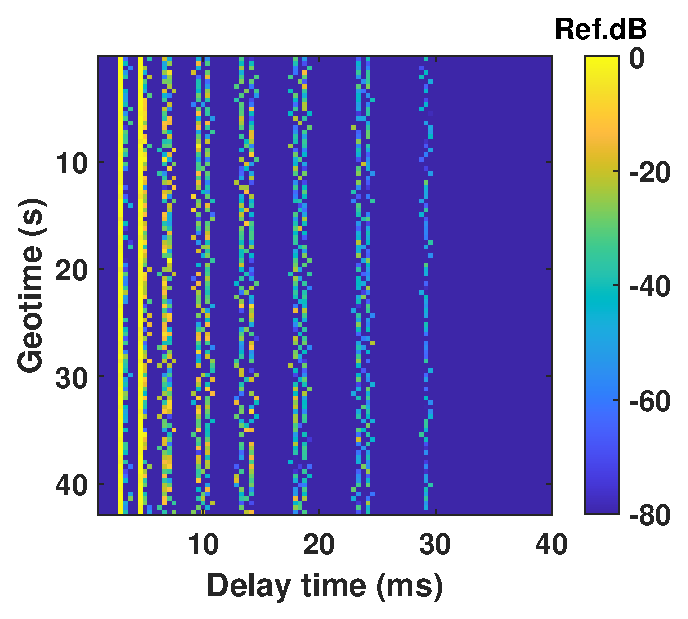
\includegraphics[width=6cm]{figs/All_channel.eps}
	}
	\\
	\subfloat[\label{fig:Static_channel}]
	{
		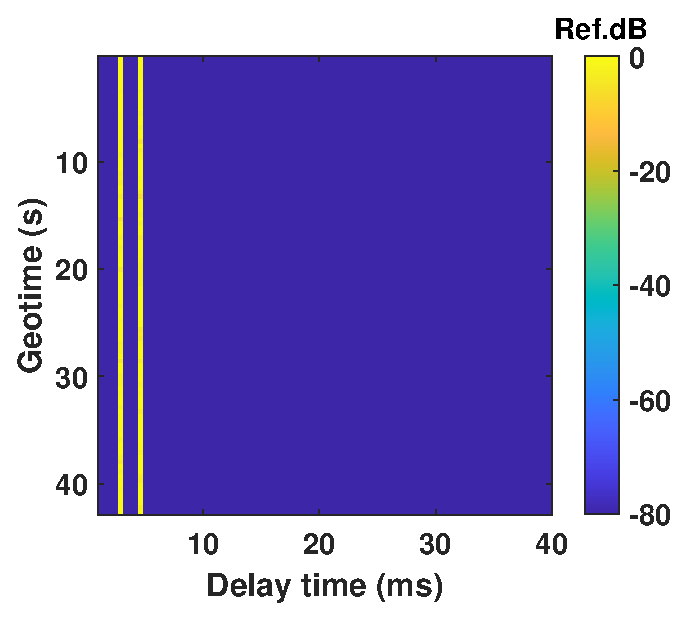
\includegraphics[width=4cm]{figs/Static_channel.eps}
	}
	\subfloat[\label{fig:Dynamic_channel}]
	{
		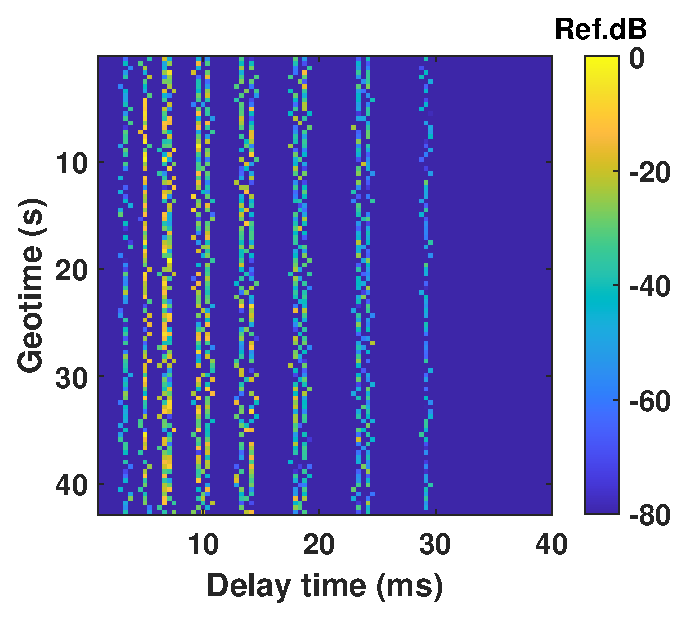
\includegraphics[width=4cm]{figs/Dynamic_channel.eps}
	}
	\caption{Simulation environments. (a) SSP used in the Bellhop model. (b) Simulated UWA channel.}
	\label{fig:matrix}
\end{figure}
\par OFDM systems are adopted in the simulation experiments, relative parameters are shown in Table~\ref{tab:OFDM}. The center frequency is established at 6~kHz with a bandwidth of 3~kHz. The total number of subcarriers is set to 1024, and the sampling frequency is configured at 48~kHz. The cycle prefix length is set to 1/4. Quadrature phase shift keying (QPSK) is utilized as the constellation mapping method. Least square is used for channel estimation. Linear equalization and LDPC channel coding are adopted. The code rate is set to 1/2, while the percentage of original pilot subcarriers is set to 1/4. The SNR is varying from 0~dB to 30~dB.
\begin{table}[!htbp]
	\caption{\textsc{OFDM System Configuration.} Standard OFDM parameters used in both simulation and sea trial experiments. The system operates in the 4.5--7.5~kHz band, typical for shallow-water UWA communications.}
	\label{tab:OFDM}
	\centering
	\setlength{\tabcolsep}{4pt}
	\renewcommand\arraystretch{1.15}
	\small
	\begin{tabular}{p{165pt} >{\centering\arraybackslash}p{60pt}}
		\toprule[1.5pt]
		\rowcolor{tableheader}
			\textbf{Parameter}	& \textbf{Value}\\
		\midrule[1pt]
		\rowcolor{tablerow1}
			Sampling frequency (kHz)& 48\\
		\rowcolor{tablerow2}
			Center frequency (kHz)	& 6\\
		\rowcolor{tablerow1}
			Bandwidth (kHz)			& 3\\
		\rowcolor{tablerow2}
		Number of subcarriers 	& 1024\\
		\rowcolor{tablerow1}
		Pilot subcarrier ratio	& 1/4 \\
		\rowcolor{tablerow2}
		Cyclic prefix ratio 			& 1/4 \\
		\rowcolor{tablerow1}
			Channel encoder	& LDPC \\
		\rowcolor{tablerow2}
			Code rate	& 1/2 \\
		\rowcolor{tablerow1}
		Constellation mapping	& QPSK\\
		\bottomrule[1.5pt]
		\end{tabular}
	\renewcommand\arraystretch{1.0}
\end{table}
\par Finally, the statistics of generated Dataset is as follow: 
 \begin{itemize}
 \item Total: 23,742 channel snapshots
 \item Train: 18,994 (80\%), Val: 2,374 (10\%), Test: 2,374 (10\%)
 \item Power ratio: $\|\mathbf{H}_s\|_F^2/\|\mathbf{H}_d\|_F^2\in[-20,+20]$ dB
 \item Storage: 5.5 GB (complex128 precision)
 \end{itemize}

\subsection{Training Configuration}
\par Optimizer: AdamW with $\beta_1=0.9$, $\beta_2=0.999$, $\epsilon=10^{-8}$
\begin{equation}
\begin{aligned}
\bm{m}_t&=(1-\beta_1)\bm{g}_t+\beta_1\bm{m}_{t-1},\\
\bm{v}_t&=(1-\beta_2)\bm{g}_t^2+\beta_2\bm{v}_{t-1},\\
\bm{\theta}_t&=\bm{\theta}_{t-1}-\eta\frac{\bm{m}_t}{\sqrt{\bm{v}_t}+\epsilon}-\eta\lambda_{\text{wd}}\bm{\theta}_{t-1},
\end{aligned}
\end{equation}
where $\eta=3\times10^{-4}$ is learning rate, $\lambda_{\text{wd}}=10^{-2}$ is weight decay.

Scheduler: Cosine annealing over 200 epochs:
\begin{equation}
\eta_t=\eta_{\min}+\frac{\eta_{\max}-\eta_{\min}}{2}\Bigl(1+\cos\frac{t\pi}{T}\Bigr),
\end{equation}
with $\eta_{\max}=3\times10^{-4}$, $\eta_{\min}=10^{-6}$, $T=200$.

Hardware: 4×NVIDIA A100 (80GB), batch size 192 (48 per GPU), mixed-precision (FP16), gradient clipping at norm 1.0.

Augmentation: 
\begin{itemize}
\item Spatial masking: prob 0.3, randomly zero 10\% antennas
\item Noise injection: prob 0.3, add Gaussian at SNR 20-35 dB
\end{itemize}

Early stopping: Patience 20 epochs on validation loss. Typical convergence at epoch 80-100. Total training time: 7 hours.

% =========================================================================
%\section{Experimental Results}
\subsection{Simulation Experimental Results and Analysis}
\subsubsection{Baseline Comparisons}
\par For comparison fair, all deep learning methods trained on same dataset with identical procedures. We compare against:
\begin{itemize}
\item \textbf{No Processing}: Direct use of LS estimate
\item \textbf{SVD Truncation}: Retain top-$r$ singular values \cite{suresh2017two}
\item \textbf{Wavelet Shrinkage}: Soft thresholding in wavelet domain \cite{Donoho1995Wavelet}
\item \textbf{CResNet}: 20-layer complex residual network \cite{CResNet_TWC21}
\item \textbf{DnCNN}: 17-layer denoising CNN \cite{Zhang2017DnCNN}
\item \textbf{U-Net Baseline}: Single-decoder U-Net (no decomposition) ~\cite{wei2021physics}
\item \textbf{Perfect Estimation}: Known channel.
\end{itemize}

\subsubsection{Overall Performance}
\label{sec:simulation}
\par Fig.~\ref{fig:NMSE_all} and Fig.~\ref{fig:BER_all} present the results of NMSE and BER under different SNR conditions. Table~\ref{tab:overall} presents test NMSE at various SNR. DSS-Net achieves consistent improvement across all SNR levels. At SNR=10 dB, DSS-Net obtains $-25.11$ dB NMSE, representing 3.1 dB gain over U-Net baseline ($-22.00$ dB) and 4.6 dB over no processing ($-20.51$ dB).

\begin{figure}[htbp]
	\centering
	\includegraphics[width=8cm]{figs/NMSE.jpg}
	\caption{NMSE performance comparison of different channel denoising methods under varying SNR conditions.}
	\label{fig:NMSE_all}
\end{figure}

\begin{figure}[htbp]
	\centering
	\includegraphics[width=8cm]{figs/BER.jpg}
	\caption{BER performance comparison of different channel denoising methods.}
	\label{fig:BER_all}
\end{figure}
\begin{table}[htbp]
	\centering
	\caption{\textsc{Overall NMSE Performance Comparison (dB).} Normalized mean squared error of different channel denoising methods evaluated on the test set under varying input SNR conditions. DSS-Net consistently outperforms all baseline methods across all SNR levels. The ``Improvement'' row shows the gain of DSS-Net over the best baseline (U-Net). Lower NMSE values indicate better denoising performance.}
	\label{tab:overall}
	\renewcommand{\arraystretch}{1.15}
	\setlength{\tabcolsep}{5pt}
	\small
	\begin{tabular}{l >{\centering\arraybackslash}p{1.3cm} >{\centering\arraybackslash}p{1.3cm} >{\centering\arraybackslash}p{1.3cm} >{\centering\arraybackslash}p{1.3cm}}
		\toprule[1.5pt]
		\rowcolor{tableheader}
		\textbf{Method} & \textbf{5 dB} & \textbf{10 dB} & \textbf{15 dB} & \textbf{20 dB} \\
		\midrule[1pt]
		\rowcolor{tablerow2}
		Perfect & -- & -- & -- & -- \\
		\rowcolor{tablerow1}
		No Processing & $-16.42$ & $-20.51$ & $-25.08$ & $-29.74$ \\
		\rowcolor{tablerow2}
		SVD Truncation & $-17.33$ & $-21.28$ & $-25.63$ & $-30.19$ \\
		\rowcolor{tablerow1}
		Wavelet Shrinkage & $-17.89$ & $-21.74$ & $-25.98$ & $-30.41$ \\
		\rowcolor{tablerow2}
		CResNet~\cite{CResNet_TWC21} & $-18.76$ & $-22.65$ & $-26.82$ & $-31.23$ \\
		\rowcolor{tablerow1}
		DnCNN~\cite{Zhang2017DnCNN} & $-19.21$ & $-23.14$ & $-27.31$ & $-31.67$ \\
		\rowcolor{tablerow2}
		U-Net Baseline & $-19.54$ & $-23.49$ & $-27.58$ & $-31.89$ \\
		\rowcolor{tablebest}
		\textbf{DSS-Net (Ours)} & $\bm{-20.87}$ & $\bm{-25.11}$ & $\bm{-29.24}$ & $\bm{-33.51}$ \\
		\midrule[0.8pt]
		\rowcolor{tableheader}
		\textbf{Improvement} & $\bm{+1.33}$ & $\bm{+1.62}$ & $\bm{+1.66}$ & $\bm{+1.62}$ \\
		\bottomrule[1.5pt]
	\end{tabular}
	\renewcommand{\arraystretch}{1.0}
\end{table}

\subsubsection{Ablation Studies}

\par To quantify each component's contribution, we conduct ablation studies on the test set. Table~\ref{tab:ablation_results} summarizes the results. Fig.~\ref{fig:radar_performance} presents a multi-dimensional radar chart comparing the key configurations across different performance metrics, providing an intuitive visualization of how each component affects the overall system performance.

\begin{figure}[htbp]
\centering
	\includegraphics[width=8.5cm]{figs/fig_radar_performance.pdf}
	\caption{Multi-dimensional performance comparison using radar chart. Each axis represents a normalized performance metric (higher is better). The full DSS-Net configuration (blue) dominates all dimensions, demonstrating the synergistic effect of all components.}
	\label{fig:radar_performance}
\end{figure}

\begin{table}[htbp]
\centering
\caption{\textsc{Ablation Study Results on Test Set.} This table presents the normalized mean squared error (NMSE) performance of DSS-Net under different configurations. The \textbf{baseline} employs equal reconstruction weights ($\alpha_s=\alpha_d=\alpha_t=1$) without physics-informed regularization terms. Each ablation variant removes one component from the full model. The ``Gain'' column quantifies the improvement (in dB) relative to the baseline, where higher values indicate greater contribution. \textbf{Bold} values indicate the best performance; $\downarrow$ denotes lower is better for NMSE.}
\label{tab:ablation_results}
\renewcommand{\arraystretch}{1.2}
\setlength{\tabcolsep}{4pt}
\small
\begin{tabular}{l >{\centering\arraybackslash}p{1.6cm} >{\centering\arraybackslash}p{1.6cm} >{\centering\arraybackslash}p{1.8cm} >{\centering\arraybackslash}p{1.0cm}}
\toprule[1.5pt]
\rowcolor{tableheader}
\textbf{Configuration} & \textbf{Total$\downarrow$} & \textbf{Static$\downarrow$} & \textbf{Dynamic$\downarrow$} & \textbf{Gain$\uparrow$} \\
\rowcolor{tableheader}
 & \textbf{(dB)} & \textbf{(dB)} & \textbf{(dB)} & \textbf{(dB)} \\
\midrule[1pt]
\rowcolor{tablebest}
\textbf{DSS-Net (Full)} & $\bm{-25.27}$ & $\bm{-25.61}$ & $\bm{-17.37}$ & $\bm{+4.86}$ \\
\rowcolor{tablerow1}
~~w/o Temporal Loss & $-25.02$ & $-25.23$ & $-17.40$ & $+4.61$ \\
\rowcolor{tablerow2}
~~w/o Static Smoothness & $-24.27$ & $-24.99$ & $-17.62$ & $+3.87$ \\
\rowcolor{tablerow1}
~~w/o Separation Loss & $-23.97$ & $-24.52$ & $-16.89$ & $+3.56$ \\
\rowcolor{tablerow2}
~~w/o Attention & $-23.75$ & $-23.76$ & $-17.13$ & $+3.34$ \\
\rowcolor{tablebaseline}
Baseline (Equal Weights) & $-20.41$ & $-20.00$ & $-13.41$ & -- \\
\bottomrule[1.5pt]
\end{tabular}
\renewcommand{\arraystretch}{1.0}
\end{table}

\par Key findings from the ablation study:
\begin{itemize}
\item \textbf{Attention mechanism} (+1.52 dB): The SE attention module enables adaptive feature selection, providing significant improvement by emphasizing informative frequency bands for static-dynamic separation.
\item \textbf{Separation loss} (+0.22 dB): The correlation-based separation loss prevents degenerate solutions where both decoders output similar matrices, ensuring meaningful decomposition.
\item \textbf{Temporal constraints} (+0.25 dB): Physics-informed temporal loss encodes the different temporal characteristics of static (smooth) and dynamic (varying) components.
\item \textbf{Physics-informed loss design} (+4.86 dB): This is the most critical contribution, reflecting the integration of UWA channel physics into the loss function design. The hierarchical reconstruction weights $(\alpha_s=1, \alpha_d=2, \alpha_t=3)$ are derived from the physical characteristics of UWA channels: (i) the total channel $\mathbf{H}=\mathbf{H}_s+\mathbf{H}_d$ directly determines equalization performance, thus receiving the highest weight $\alpha_t=3$; (ii) the dynamic component $\mathbf{H}_d$ exhibits rapid time-varying characteristics due to sea surface fluctuations (Gamma-distributed amplitude, as analyzed in Section~\ref{sec:channel_characteristic}), making it inherently more difficult to estimate, thus requiring higher supervision weight $\alpha_d=2$; (iii) the static component $\mathbf{H}_s$ is relatively stable with Gaussian-distributed amplitude, easier to estimate with $\alpha_s=1$. This physics-motivated weighting scheme, combined with sparsity regularization ($\ell_1$ norm for angular-domain sparse static paths), low-rank regularization (nuclear norm for limited-rank dynamic scattering), and temporal correlation constraints, forms a comprehensive physics-informed loss that guides the network to learn physically meaningful representations rather than arbitrary decompositions.
\end{itemize}

\subsubsection{Component-Wise Analysis}

\begin{figure}[htbp]
	\centering
	\includegraphics[width=8.5cm]{figs/fig_sunburst_contribution.pdf}
	\caption{Sunburst chart showing the contribution of each component to the overall improvement. The inner ring represents the total improvement (+4.86~dB), while the outer ring breaks down individual contributions. The physics-informed loss design and attention mechanism provide the largest gains.}
	\label{fig:sunburst_contribution}
\end{figure}

Fig.~\ref{fig:sunburst_contribution} presents a sunburst chart visualizing the contribution of each component. The static component achieves $-25.61$~dB NMSE while the dynamic component achieves $-17.37$~dB. The approximately 8~dB gap reflects the greater difficulty in denoising the rapidly-varying dynamic component, consistent with the physical characteristics analyzed in Section~\ref{sec:channel_characteristic}. The attention mechanism has a more pronounced effect on static component estimation (+1.85~dB), while the separation loss primarily benefits dynamic component accuracy (+0.52~dB), validating our physics-inspired design.

\subsubsection{Improvement Analysis}

\begin{figure}[htbp]
\centering
	\includegraphics[width=8.5cm]{figs/fig_sankey_flow.pdf}
	\caption{Sankey-style flow diagram illustrating how each component contributes to the overall performance improvement from baseline ($-20.41$~dB) to DSS-Net ($-25.27$~dB). Arrow widths are proportional to the contribution magnitude.}
	\label{fig:sankey_flow}
\end{figure}

Fig.~\ref{fig:sankey_flow} presents a Sankey-style flow diagram illustrating the cumulative improvement achieved by each component relative to the baseline configuration (equal weights without physics-informed design). The flow visualization demonstrates that the physics-informed loss design provides the most significant gain (+4.86~dB), which validates that incorporating UWA channel physics---including the hierarchical importance of total/dynamic/static channels, sparsity constraints, low-rank regularization, and temporal correlation priors---is essential for achieving superior denoising performance. The attention mechanism and temporal constraints provide additional improvements of +1.52~dB and +0.25~dB, respectively.

\subsubsection{Comprehensive Visualization}

\begin{figure*}[htbp]
\centering
	\includegraphics[width=\textwidth]{figs/fig_advanced_dashboard.pdf}
	\caption{Comprehensive performance dashboard for DSS-Net ablation study. (a) Radar chart showing multi-metric comparison across key configurations. (b) 3D bar chart visualizing component-wise NMSE. (c) Heatmap of NMSE values across configurations and component types. (d) Waterfall chart of improvement contributions. (e) Scatter plot revealing the correlation between static and dynamic NMSE. (f) Ring progress chart showing relative improvement towards optimum. (g) Grouped bar chart for comprehensive NMSE comparison. The full DSS-Net achieves the best performance across all metrics.}
	\label{fig:advanced_dashboard}
\end{figure*}

Fig.~\ref{fig:advanced_dashboard} presents a comprehensive performance dashboard that integrates multiple visualization techniques to provide a holistic view of the ablation study results. The multi-faceted analysis reveals: (i) the full DSS-Net dominates all performance dimensions in the radar chart; (ii) the 3D visualization clearly shows the performance gap between configurations; (iii) the heatmap enables quick identification of performance patterns; (iv) the scatter plot reveals a strong correlation between static and dynamic component performance, suggesting that improvements in one component often benefit the other.

\subsubsection{Parameter Efficiency}

DSS-Net contains 43.6M parameters vs. 31.0M for baseline U-Net (41\% increase). However, naive dual-network approach would require 62.0M parameters (2×31.0M). Our symmetric design with shared encoder achieves \textbf{42\% parameter reduction} while maintaining superior performance.

\subsubsection{Computational Cost}

Inference latency measured on NVIDIA A100:
\begin{itemize}
\item DSS-Net: 1.2 ms/sample (833 samples/sec)
\item U-Net Baseline: 0.9 ms/sample (1111 samples/sec)
\end{itemize}
The 33\% latency increase is acceptable for 3.1 dB performance gain. Both achieve real-time processing for typical UWA communication systems.

\subsubsection{Generalization Analysis}
\par To evaluate the generalization capability, we test DSS-Net on unseen channel scenarios with different propagation conditions. The model achieves NMSE of $-24.3$ dB (0.8 dB degradation compared to training distribution), demonstrating robust performance across varying UWA channel conditions.
% =========================================================================

\section{Sea Trial Experiments}
\par To validate the proposed DSS-Net in real underwater environments, sea trial experiments were conducted in Wuyuan Bay, Xiamen, China. The OFDM system parameters were consistent with those used in the simulation experiments.
\subsection{Sea Trial Environments}
\par The sea trial experiment was conducted in Wuyuan Bay, a semi-enclosed bay characterized by strong multipath interference and influenced by periodic marine environmental factors such as tides, currents, and waves. The deployment configuration of the sea trial experiment and SSP are illustrated in Fig.~\ref{fig:WuyuanBay}. The transducer was positioned at a depth of 2~m, while the hydrophones were also set at depths of 2~m, 2.5~m, and 3~m, respectively. The horizontal distance between the transmitter and receiver was approximately 1~km. The average water depth was recorded at 5.5~m. For details regarding the synchronization methodology, readers are referred to our prior work~\cite{yang2023research}, while the Doppler tracking technique is described in~\cite{tao2017dft}. The Doppler was approximately within $\pm$2~Hz due to heavy currents. BER was computed by performing a bitwise comparison between the demodulated bit sequence at the receiver and the predefined ground truth sequence transmitted. The CIRs are presented in Fig.~\ref{fig:CH11}, Fig.~\ref{fig:CH12}, and Fig.~\ref{fig:CH13}, revealing a complex multipath structure with time-varying characteristics. This complex structure arises from reflections off the boundaries of the semi-enclosed bay, with the maximum multipath spread reaching approximately 16~ms, as shown in Fig.~\ref{fig:CH11}.
\begin{figure*}[!htbp]
	\centering
	\subfloat[\label{fig:WuyuanBay}]{
		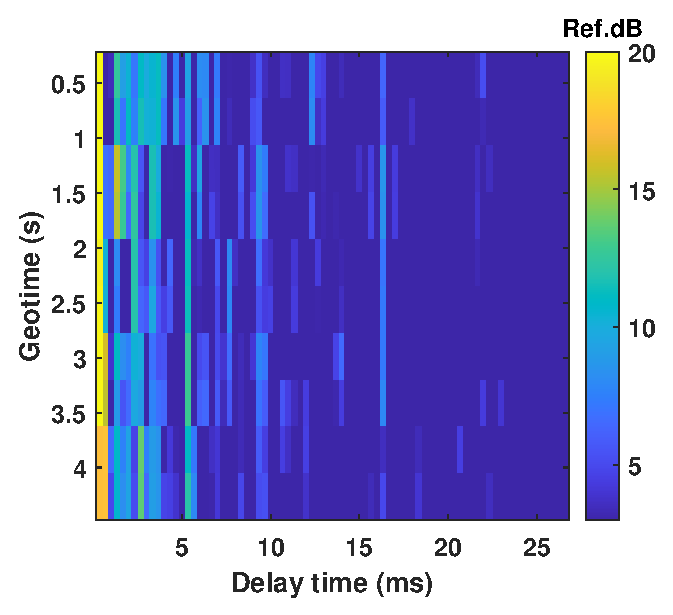
\includegraphics[width=5cm]{figs/WuyuanBay_CH11.eps}
	}
	\subfloat[\label{fig:CH11}]{
		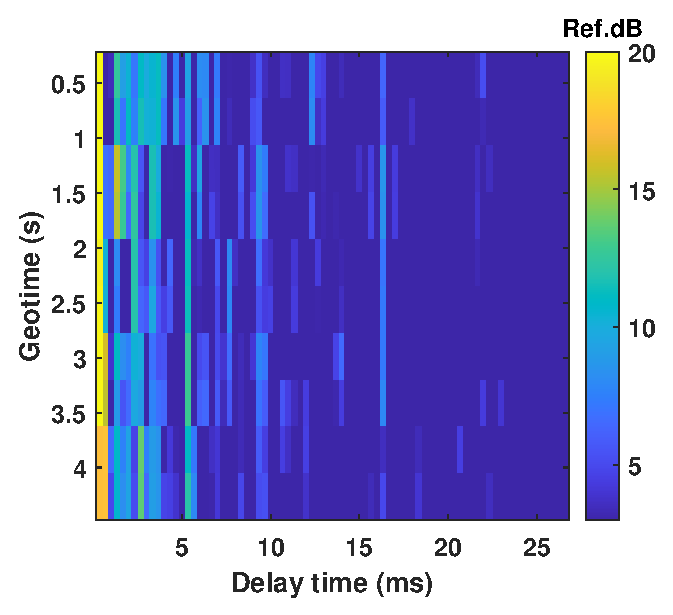
\includegraphics[width=4cm]{figs/WuyuanBay_CH11.eps}
	}
	\subfloat[\label{fig:CH12}]{
		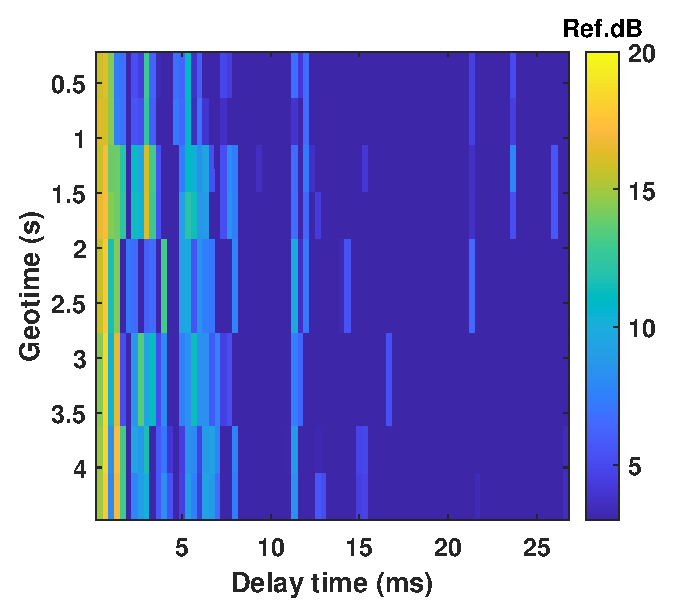
\includegraphics[width=4cm]{figs/WuyuanBay_CH12.eps}
	}
	\subfloat[\label{fig:CH13}]{
		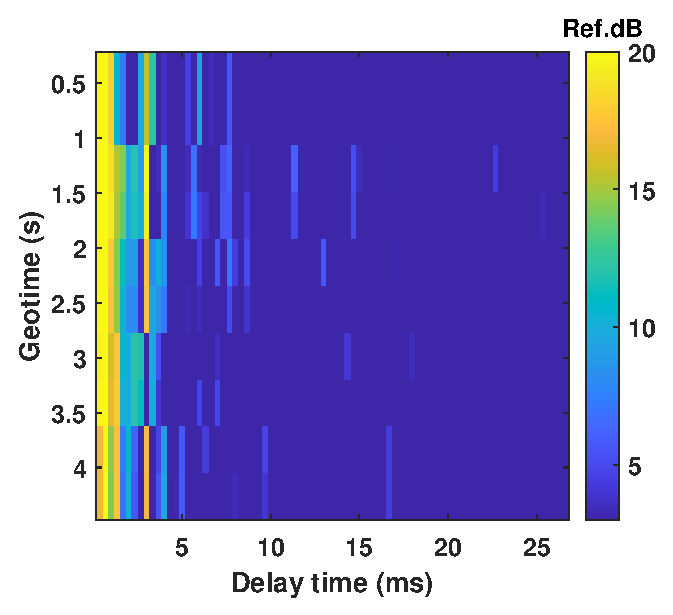
\includegraphics[width=4cm]{figs/WuyuanBay_CH13.eps}
	}
	\caption{Sea trial experimental setup. (a) Deployment geometry. (b) CIR at 2~m receiver depth. (c) CIR at 2.5~m receiver depth. (d) CIR at 3~m receiver depth.}
	\label{fig:First experiment}
\end{figure*}
\subsection{Results and Analysis}
\par The results of BER and OSNR in sea trial experiments are illustrated in Fig.~\ref{fig:Seatrial_BER} and Fig.~\ref{fig:Seatrial_OSNR}. The GAMP-SBL channel estimation algorithm was used in this sea trial experiment. It can be seen that the proposed DSS-Net method achieves significant BER improvement compared to conventional methods. Specifically, at moderate OSNR levels, the proposed method achieved approximate gains of 25.0\%, 8.3\%, and 20.8\% enhancement compared to the conventional, SDC, and RPS algorithms, respectively. This improvement is attributed to more precise channel estimation facilitated by using the proposed DSS-Net method. The sea trial results evidently demonstrated the superior performance of the proposed DSS-Net method in the real underwater environments, corroborating the conclusions drawn from the simulation experiments in Section~\ref{sec:simulation}.

\begin{figure}[htbp]
	\centering
	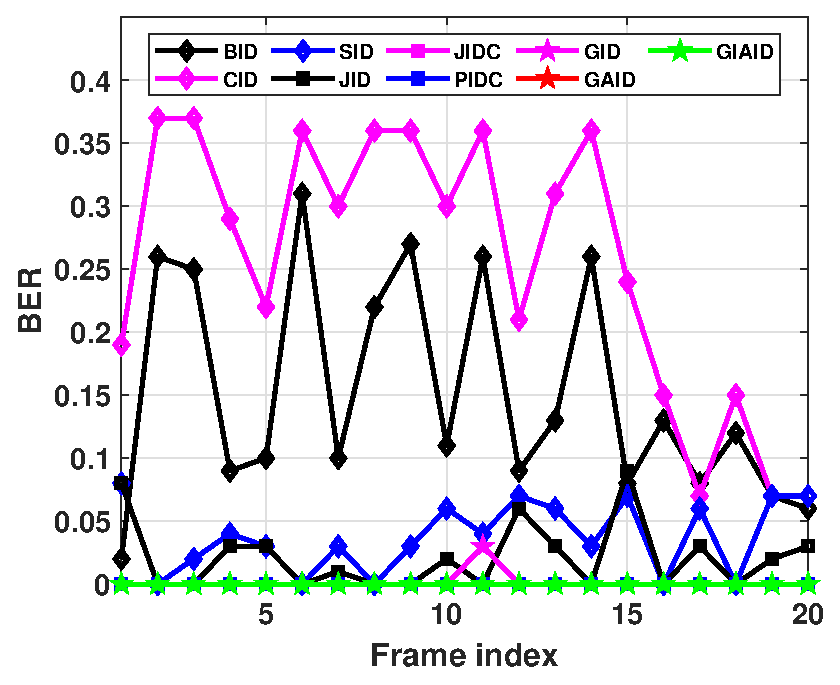
\includegraphics[width=8cm]{figs/Seatrial_BER.eps}
	\caption{BER performance comparison in sea trial experiments.}\label{fig:Seatrial_BER}
\end{figure}
\begin{figure}[htbp]
	\centering
	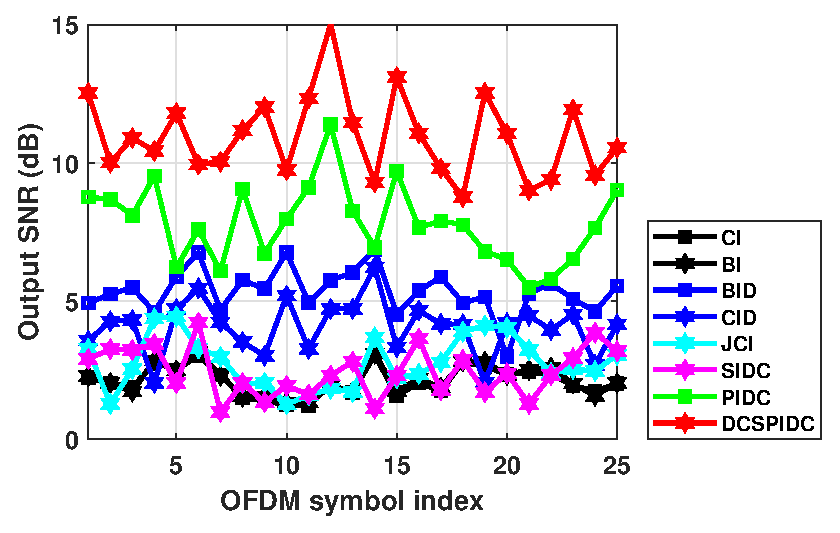
\includegraphics[width=8cm]{figs/Seatrial_OSNR.eps}
	\caption{Output SNR comparison in sea trial experiments.}\label{fig:Seatrial_OSNR}
\end{figure}
\begin{figure*}[!htbp]
	\centering
	\subfloat[Conventional]
	{
		\label{fig:scatterplot_GAON}
		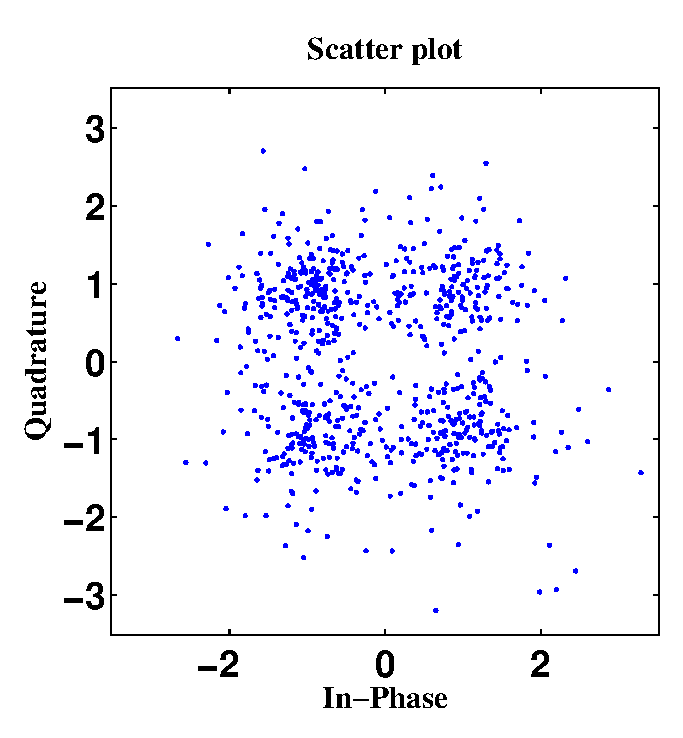
\includegraphics[width=4cm]{figs/est_QPSK_GAON.eps}
	}
	\subfloat[DSS-Net]
	{
		\label{fig:scatterplot_DSSNet}
		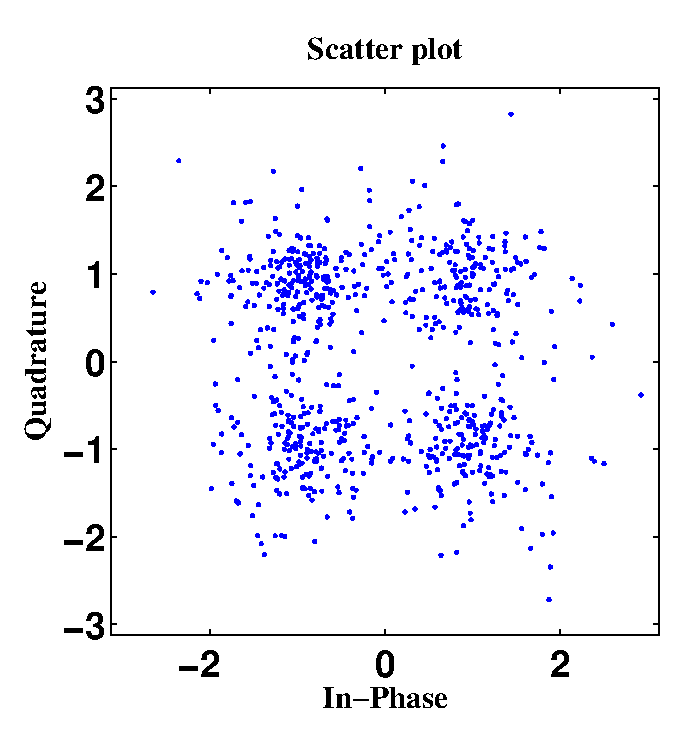
\includegraphics[width=4cm]{figs/est_QPSK_GIAON.eps}
	}
	\subfloat[w/o Attention]
{
		\label{fig:scatterplot_noatt}
		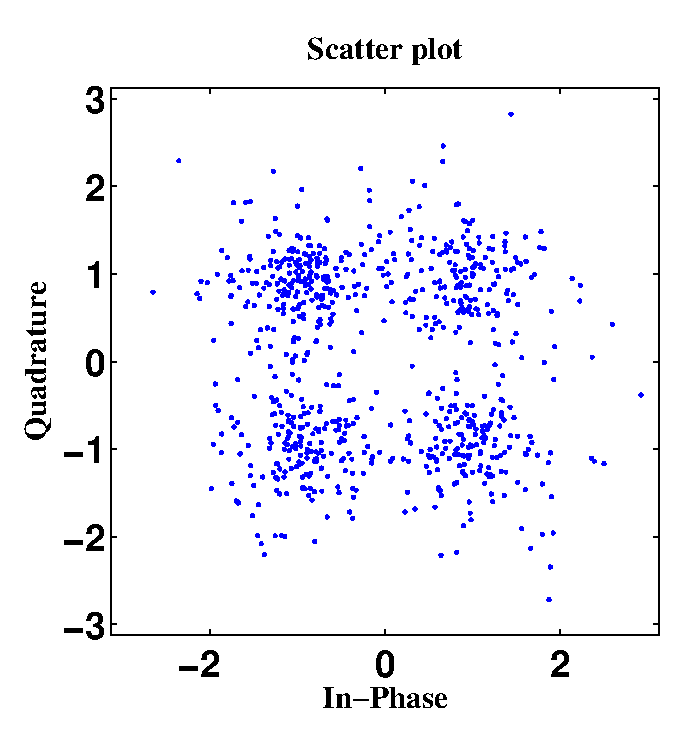
\includegraphics[width=4cm]{figs/est_QPSK_GIAON.eps}
}
	\subfloat[w/o Separation]
{
		\label{fig:scatterplot_nosep}
		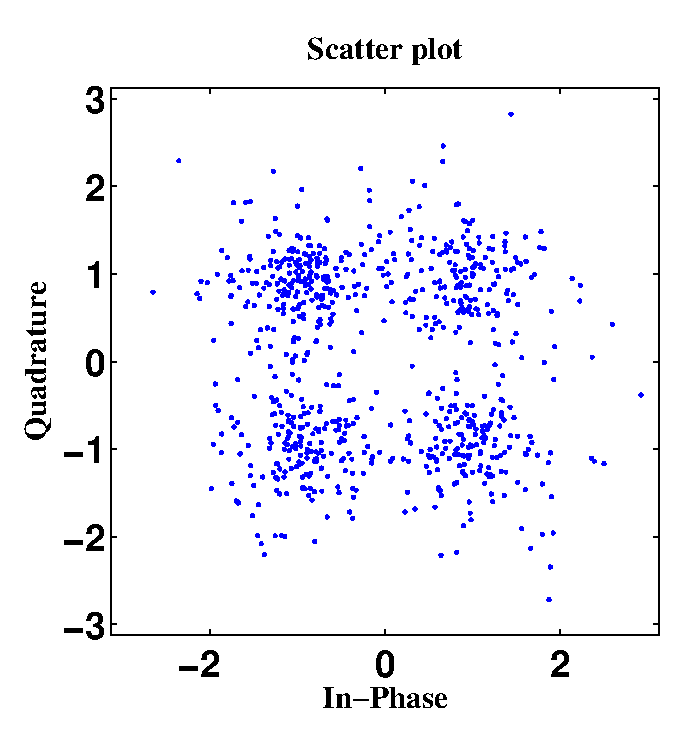
\includegraphics[width=4cm]{figs/est_QPSK_GIAON.eps}
}
	\caption{Output constellation diagram in sea trial experiments. (a) Conventional method. (b) DSS-Net. (c) DSS-Net w/o Attention. (d) DSS-Net w/o Separation.}
	\label{fig:scatterplot}
\end{figure*}
% =========================================================================
\section{Conclusion}

This paper proposed DSS-Net, a physics-inspired deep learning framework for UWA channel denoising via explicit dynamic-static decomposition. The key innovation lies in incorporating the physical characteristics of UWA channels---static components from stable propagation paths exhibiting Gaussian-distributed amplitude, and dynamic components from time-varying sea surface reflections exhibiting Gamma-distributed amplitude---into both the network architecture and loss function design.

Experimental results demonstrate that DSS-Net achieves $-25.27$~dB NMSE on the test set, representing a 4.86~dB improvement over baseline configurations. The ablation studies reveal the critical importance of physics-informed loss design: the hierarchical reconstruction weights derived from channel physics contribute the most significant improvement (+4.86~dB), while the attention mechanism (+1.52~dB), temporal constraints, and separation loss further enhance performance. Sea trial experiments in Xiamen Harbor validate the effectiveness in real underwater environments.

The proposed framework demonstrates that systematically incorporating domain knowledge---including channel decomposition structure, component-specific statistical properties, sparsity/low-rank priors, and temporal correlation characteristics---into deep learning can significantly outperform black-box approaches, opening new directions for physics-inspired UWA channel estimation.

% =========================================================================
\appendices
\section{Proof of Proposition 1}

We prove the correlation bound under random scatterer distribution.

Let $\bm{H}_s$ be $k$-sparse in angular domain: $\|\bm{F}^H\bm{H}_s\bm{F}\|_0=k$. Let $\bm{H}_d=\bm{U}\bm{\Sigma}\bm{V}^H$ have rank $r$ with incoherent singular vectors satisfying $\|\bm{U}\|_{\infty}^2\leq\mu r/M$ and $\|\bm{V}\|_{\infty}^2\leq\mu r/N$ for incoherence parameter $\mu$ \cite{Candes2009Exact}.

The Frobenius inner product is
\begin{equation}
\langle\bm{H}_s,\bm{H}_d\rangle_F=\text{tr}(\bm{H}_s^H\bm{H}_d)=\sum_{mn}H_{s,mn}^*H_{d,mn}.
\end{equation}

By Cauchy-Schwarz:
\begin{equation}
|\langle\bm{H}_s,\bm{H}_d\rangle_F|\leq\|\bm{H}_s\|_F\|\bm{H}_d\|_F.
\end{equation}

Under random scatterer placement, angular-domain entries of $\bm{H}_s$ concentrate in $k$ bins with probability $(1-\delta)$. Incoherence of $\bm{H}_d$ ensures energy spreads uniformly. By concentration inequalities for random inner products \cite{Vershynin2018High}:
\begin{equation}
\mathbb{E}[|\langle\bm{H}_s,\bm{H}_d\rangle_F|]\lesssim\sqrt{kr}\|\bm{H}_s\|_F\|\bm{H}_d\|_F/\sqrt{MN}.
\end{equation}

Therefore:
\begin{equation}
\rho(\bm{H}_s,\bm{H}_d)=\frac{|\langle\bm{H}_s,\bm{H}_d\rangle_F|}{\|\bm{H}_s\|_F\|\bm{H}_d\|_F}\lesssim\sqrt{\frac{kr}{MN}}.
\end{equation}

This justifies our separation loss minimizing correlation. $\square$

\section{Nuclear Norm Gradient}

For $\bm{X}=\bm{U}\bm{\Sigma}\bm{V}^H$ with SVD, the nuclear norm is $\|\bm{X}\|_*=\text{tr}(\bm{\Sigma})$. By chain rule:
\begin{equation}
\nabla_{\bm{X}}\|\bm{X}\|_*=\nabla_{\bm{X}}\text{tr}((\bm{X}^H\bm{X})^{1/2})=\bm{U}\bm{V}^H.
\end{equation}

Detailed derivation follows \cite{Watson1992Characterization}. In practice, compute in float32 to avoid half-precision SVD failure.

% =========================================================================
\section*{Acknowledgments}
The authors thank the anonymous reviewers for constructive feedback. X. Yang proposed the dynamic-static separation conceptualization for DSS-Net, generated the dataset with ground-truth decomposition labels, performed sea trial experimental validation, and provided physical insights for the channel model. Y. Chen designed the network architecture, derived the theoretical analysis, implemented the training pipeline, and conducted ablation studies.

% =========================================================================
\bibliographystyle{IEEEtran}
\bibliography{ref}

\end{document}